% Appendix E: details of Claim 2 (a match at the later mention, read by key). Input by sections/appendix.tex.
\section{A match at the later mention, read by key: details}\label{app:claim2}

This appendix gives the discovery-sample results on which later tokens read the writing token's key and through which heads (\cref{app:readers,app:heads}; preregistrations D, G and H), and the final round's tests of what those heads write (\cref{app:flag}), what sets the sign of the read (\cref{app:sign}) and how the flag behaves across scale (\cref{app:scale}). The final round's mechanism tests use Qwen2.5-7B and Mistral-7B (and Qwen2.5-1.5B and 3B for scale), the reader heads frozen from the discovery sample, flags fit on its 60 ranking stories and 100 new evaluation stories; intervals are 95\,\% story-bootstrap intervals, and a line over the two 7B models holds only if it holds in both.

\subsection{The mechanism tests in brief}\label{app:claim2-brief}

This subsection gives, verbatim, the fuller account of the mechanism tests that the reporting plan placed in the main text (moved here; \cref{sec:claim2} gives a shorter one; the move is disclosed in \cref{app:decisions}, deviation (iv)). The status marks are those of the main text (\cref{sec:method}); the subsections below give every number.

\textbf{In two 7B models (Qwen2.5-7B, Mistral-7B), the reader heads, enriched for duplicate-token heads (discovery sample), match the writing token's key at the later mention of the written value and write a flag into that mention's row, which the answer reads by key.} The flag suffices to move the answer but is neither specific nor the only carrier, and the question sets the sign of the read.

\paragraph{Two hops.}
In the discovery sample, 5\,\% of heads, the \emph{reader heads}, read the writing token's key at the option words (hop~1): seeing the clamped key alone, they recover \HoneRQwenSeven{} and \HoneRMistralSeven{} of the option rows' read, random sets almost none, and no single head or layer carries most of the read (\cref{app:heads}). They are enriched for duplicate-token heads \citep{wang2022ioi}: the \HfourKCQwenSeven{} and \HfourKCMistralSeven{} heads carrying 80\,\% of the read have median duplicate-token scores of \HfourDQwenSeven{} and \HfourDMistralSeven{}, against \HfourDwholeQwenSeven{} and \HfourDwholeMistralSeven{} over all heads (exploratory), a core that depends on how many heads are counted. Mean-ablating all reader heads at the option rows leaves \HthreeRhoQwenSeven{} and \HthreeRhoMistralSeven{} of the key read and raises the value read: a copy route stays available (\cref{app:heads}). The answer reads the option words, not the writing token (hop~2), mainly by key.

\paragraph{What the readers write.}
The reader heads write one vector per layer into the re-mentioned word's row. We call it the \emph{flag}. Injected with no key clamp into the row of an option absent from the story, a version fit without that word moves the answer there (\JdOneRatioQwenSeven{} / \JdOneRatioMistralSeven{} of the key read's identity effect; the answer changes in \pct{\JdOnePiXQwenSeven} / \pct{\JdOnePiXMistralSeven} of stories)\rsk. Like the natural key clamp, the injection adds the flag at that row and removes it at the base value's row; added alone, one flag moves the answer less than the natural clamp, half a flag almost not at all (exploratory; \cref{fig:flag}a). Its mean direction names no candidate: fit under the key-only clamp or from the natural source run, it is the same direction with the same effect, although each story's write also carries its word (exploratory; \cref{app:flag}). The answer reads it by key, as it reads the natural one (giving only the answer row the option rows' original keys removes \JdFourKQwenSeven{} / \JdFourKMistralSeven{} of its effect, their original values \JdFourVQwenSeven{} / \JdFourVMistralSeven{}). But the prediction\rsk{} that it is specific failed against structured controls: at Qwen2.5-7B the mean reader output moves the answer \JdTwoRatioMeanHQwenSeven{} as much as the flag, and at Mistral-7B the story's own write with its flag component removed, norm-matched, \JdTwoRatioOrthMistralSeven{} as much (the mean output contains the flag by construction, post hoc; \cref{app:flag}). And one direction per layer does not carry the key read ($\rho_K$ = \JdThreeRhoFlagQwenSeven{} / \JdThreeRhoFlagMistralSeven{}): other carriers exist; the flag is sufficient but not necessary (\cref{fig:flag}b). Removing the flag direction leaves about half of the key read in both models, as the prediction\rsk{} allowed; it failed on its controls: at Qwen the control directions, which overlap the flag, also remove 31\,\% and 44\,\%, and ablating the whole heads removes far more (above), so the flag is not the only carrier (\cref{app:decisions}). % verbatim: outcome J part D

\paragraph{The sign of the read.}
Asked which option was \emph{not} mentioned, both reads turn negative ($\mathrm{ID}_K$ $\fpeval{round(\JdSevenQoutQwenSeven,1)}$ and $\fpeval{round(\JdSevenQoutMistralSeven,1)}$ nats), and the same frozen reader heads carry the reads under both questions (\cref{app:sign}); the flag fit with the belief question, injected under this one, reproduces its negative effect (exploratory), so the sign is applied after the first hop. In indirect-object identification (IOI) with the names re-mentioned in a parenthesis, the key read is negative and the value read positive in both models (\cref{fig:flag}c). The negative IOI read is applied at the answer's key read of the listed names (restoring their keys and values for the answer row alone removes \JdRouteKVQwenSeven{} / \JdRouteKVMistralSeven{} of it, their keys alone \JdRouteKQwenSeven{} / \JdRouteKMistralSeven{}, their values alone \JdRouteVQwenSeven{} / \JdRouteVMistralSeven{})\rsk. The prediction\rsk{} that the ten answer-side heads ranked as the flag's top readers in lists apply it failed: a different (or a distributed) reader applies the negative read (the scoring script's reading: ``different reader''), though even in lists these ten carry only part of hop~2. That the belief readers carry the IOI read\rsk{} was met at Qwen2.5-7B and is not evaluable at Mistral-7B. The flag is written in sentences as in lists at 1.5B--7B, but four further predictions\rsk{} did not hold: that it carries the size of the sentence read across scale and is read by value at 1.5B (the preregistered decision table gives ``Mixed.''; post hoc, on a contrast specific to the absent option, the injected flag reproduces the natural ratio; \cref{app:scale}), that the initial-state flag carries binding separably from order, and that a key naming no candidate acts as removing the base value's flag.

\subsection{Which later tokens read, and what a re-mention must be}\label{app:readers}\label{sec:readers}\label{sec:forms}\label{app:stage5}

Letting only the option words see the source key recovers \locScaleOptMin{}--\locScaleOptMax{} of the full key effect at 7--14B under \fmtOpt{}, and every other group at most \locScaleOptOtherMax{}; under \fmtPost{} the sentence's candidate words recover \locScalePostMin{}--\locScalePostMax{} (D3, met; \cref{fig:readers}a). Conversely, forbidding the six candidate words to attend to the writing token removes the key identity ($r_K$, the fraction left, is $\GfiveRKMin$ to \GfiveRKMax{} in 9/9 format--model cells; G5, met), and cutting a matched control column does not (G6, met). The words must name the candidates at stake: listing B with two other candidates instead of S and X gives no read (G9, met). In lists two named candidates suffice (G10, met for lists); in sentences the read grows with the number named (G10, not met for sentences), and with only S and X named the words carry \GtwelveStwoQwenFourteen{}--\GtwelveStwoQwenSeven{} of the splice effect, most of it not identity-specific (G12, not met; \cref{app:g-membership}). The candidate words are thus the main readers in lists and in sentences naming at least three candidates.

\paragraph{What a re-mention must be.} Varying the re-mentions of \fmtPost{} in four 7--14B models shows a read of the word form, largely up to case ($r_K$: $\mathrm{ID}_K$ relative to an exact repeat). Capitalised and upper-case forms read nearly fully (\GfourteenCaseMin{}--\GfourteenCaseMax{}; G14, which predicted at most 0.75, not met), but a modified noun phrase such as ``wooden shelf'' reads only partly (\GthirteenModifMin{}--\GthirteenModifMax{}; G13, not met). Synonyms and mixed-language translations carry little on our English-scored measure (at most \GfifteenRKMax{}; G15, met). No preregistered token or concept outcome holds (G16, not met). Where the read is lost, the value identity rises (G17, met), but no more than after a sentence naming other words (exploratory; \cref{app:g-forms}).

\paragraph{Localisation.} \Cref{tab:localisation} gives the row-restricted splice for each token group. The later-mention words are the listed options under \fmtOpt{} and \fmtLetter{}, and the candidate words of the neutral sentence under \fmtPost{}. Under \fmtOpt{}, the question, the story after the writing token and the remaining tokens, including the answer position, each recover at most \locScaleOptOtherMax{} at 7--14B. Under \fmtPost{} the ``other later tokens'' recover \locScalePostOtherMin{}--\locScalePostOtherMax{}, and \locScalePostLeftMin{}--\locScalePostLeftMax{} of the effect is recovered by no single group, so the groups do not add up. At Mistral-Small-24B, with the key clamped from block~6, the option rows carry \IgtwoRatioOpt{}, \IgtwoRatioLetter{} and \IgtwoRatioPost{} of the key effect under \fmtOpt{}, \fmtLetter{} and \fmtPost{} (Gate I-G2, a head splice over all heads; \cref{app:stage7}); we did not localise the read at 72B. An earlier exploratory run at Qwen2.5-1.5B gives the same picture: the option words recover \locOptChoicewords{} of the key effect under \fmtOpt{} and \locLetterChoicewords{} under \fmtLetter{}. Restricting the splice further, the read is concentrated in layers 4--15 of 28, and one of the two KV groups carries most of it (exploratory; \cref{tab:windows}).

\begin{table}[!ht]
\centering
\caption{\textbf{Which later tokens read the writing token's key.} Fraction of the full key effect (all tokens see the source key, in every layer) recovered when only one group of later tokens sees it; ratio of mean log-odds changes. ``Other later tokens'' covers the instruction, chat template, prefill and answer position. Qwen2.5-7B, Qwen2.5-14B and Mistral-7B: BF16, $n = 60$ stories per format; preregistration D (D3) for \fmtOpt{} and \fmtPost{}, \fmtLetter{} exploratory. Qwen2.5-1.5B: FP32, $n = 40$, exploratory. 95\% bootstrap CIs. The groups need not add up to one.}
\label{tab:localisation}
{\small\begin{tabular}{llcccc}
\toprule
Model & Format & later-mention words & question & story after writing token & other later tokens \\
\midrule
Qwen2.5-1.5B & \fmtOpt{} & \begin{tabular}[t]{@{}c@{}}+0.87\\[-1pt]{\scriptsize[+0.80, +0.95]}\end{tabular} & \begin{tabular}[t]{@{}c@{}}0.00\\[-1pt]{\scriptsize[$-$0.01, +0.01]}\end{tabular} & \begin{tabular}[t]{@{}c@{}}$-$0.01\\[-1pt]{\scriptsize[$-$0.01, 0.00]}\end{tabular} & \begin{tabular}[t]{@{}c@{}}0.00\\[-1pt]{\scriptsize[$-$0.04, +0.03]}\end{tabular} \\
Qwen2.5-1.5B & \fmtLetter{} & \begin{tabular}[t]{@{}c@{}}+0.98\\[-1pt]{\scriptsize[+0.96, +1.00]}\end{tabular} & \begin{tabular}[t]{@{}c@{}}+0.01\\[-1pt]{\scriptsize[0.00, +0.01]}\end{tabular} & \begin{tabular}[t]{@{}c@{}}0.00\\[-1pt]{\scriptsize[$-$0.01, 0.00]}\end{tabular} & \begin{tabular}[t]{@{}c@{}}0.00\\[-1pt]{\scriptsize[0.00, 0.00]}\end{tabular} \\
\midrule
Qwen2.5-7B & \fmtOpt{} & \begin{tabular}[t]{@{}c@{}}+0.92\\[-1pt]{\scriptsize[+0.90, +0.94]}\end{tabular} & \begin{tabular}[t]{@{}c@{}}0.00\\[-1pt]{\scriptsize[0.00, 0.00]}\end{tabular} & \begin{tabular}[t]{@{}c@{}}0.00\\[-1pt]{\scriptsize[0.00, 0.00]}\end{tabular} & \begin{tabular}[t]{@{}c@{}}+0.01\\[-1pt]{\scriptsize[+0.01, +0.02]}\end{tabular} \\
Qwen2.5-7B & \fmtLetter{} & \begin{tabular}[t]{@{}c@{}}+1.00\\[-1pt]{\scriptsize[+0.99, +1.01]}\end{tabular} & \begin{tabular}[t]{@{}c@{}}0.00\\[-1pt]{\scriptsize[0.00, 0.00]}\end{tabular} & \begin{tabular}[t]{@{}c@{}}0.00\\[-1pt]{\scriptsize[0.00, 0.00]}\end{tabular} & \begin{tabular}[t]{@{}c@{}}0.00\\[-1pt]{\scriptsize[0.00, 0.00]}\end{tabular} \\
Qwen2.5-7B & \fmtPost{} & \begin{tabular}[t]{@{}c@{}}+0.67\\[-1pt]{\scriptsize[+0.60, +0.73]}\end{tabular} & \begin{tabular}[t]{@{}c@{}}0.00\\[-1pt]{\scriptsize[0.00, +0.01]}\end{tabular} & \begin{tabular}[t]{@{}c@{}}$-$0.01\\[-1pt]{\scriptsize[$-$0.01, 0.00]}\end{tabular} & \begin{tabular}[t]{@{}c@{}}+0.11\\[-1pt]{\scriptsize[+0.09, +0.13]}\end{tabular} \\
\midrule
Qwen2.5-14B & \fmtOpt{} & \begin{tabular}[t]{@{}c@{}}+0.94\\[-1pt]{\scriptsize[+0.93, +0.96]}\end{tabular} & \begin{tabular}[t]{@{}c@{}}0.00\\[-1pt]{\scriptsize[0.00, 0.00]}\end{tabular} & \begin{tabular}[t]{@{}c@{}}0.00\\[-1pt]{\scriptsize[0.00, 0.00]}\end{tabular} & \begin{tabular}[t]{@{}c@{}}+0.01\\[-1pt]{\scriptsize[+0.01, +0.01]}\end{tabular} \\
Qwen2.5-14B & \fmtLetter{} & \begin{tabular}[t]{@{}c@{}}+1.00\\[-1pt]{\scriptsize[+1.00, +1.00]}\end{tabular} & \begin{tabular}[t]{@{}c@{}}0.00\\[-1pt]{\scriptsize[0.00, 0.00]}\end{tabular} & \begin{tabular}[t]{@{}c@{}}0.00\\[-1pt]{\scriptsize[0.00, 0.00]}\end{tabular} & \begin{tabular}[t]{@{}c@{}}0.00\\[-1pt]{\scriptsize[0.00, 0.00]}\end{tabular} \\
Qwen2.5-14B & \fmtPost{} & \begin{tabular}[t]{@{}c@{}}+0.72\\[-1pt]{\scriptsize[+0.64, +0.80]}\end{tabular} & \begin{tabular}[t]{@{}c@{}}0.00\\[-1pt]{\scriptsize[0.00, 0.00]}\end{tabular} & \begin{tabular}[t]{@{}c@{}}0.00\\[-1pt]{\scriptsize[0.00, 0.00]}\end{tabular} & \begin{tabular}[t]{@{}c@{}}+0.09\\[-1pt]{\scriptsize[+0.07, +0.10]}\end{tabular} \\
\midrule
Mistral-7B & \fmtOpt{} & \begin{tabular}[t]{@{}c@{}}+0.98\\[-1pt]{\scriptsize[+0.96, +0.99]}\end{tabular} & \begin{tabular}[t]{@{}c@{}}0.00\\[-1pt]{\scriptsize[0.00, 0.00]}\end{tabular} & \begin{tabular}[t]{@{}c@{}}0.00\\[-1pt]{\scriptsize[0.00, 0.00]}\end{tabular} & \begin{tabular}[t]{@{}c@{}}+0.01\\[-1pt]{\scriptsize[0.00, +0.01]}\end{tabular} \\
Mistral-7B & \fmtLetter{} & \begin{tabular}[t]{@{}c@{}}+1.00\\[-1pt]{\scriptsize[+1.00, +1.01]}\end{tabular} & \begin{tabular}[t]{@{}c@{}}0.00\\[-1pt]{\scriptsize[0.00, 0.00]}\end{tabular} & \begin{tabular}[t]{@{}c@{}}0.00\\[-1pt]{\scriptsize[0.00, 0.00]}\end{tabular} & \begin{tabular}[t]{@{}c@{}}0.00\\[-1pt]{\scriptsize[0.00, 0.00]}\end{tabular} \\
Mistral-7B & \fmtPost{} & \begin{tabular}[t]{@{}c@{}}+0.73\\[-1pt]{\scriptsize[+0.67, +0.78]}\end{tabular} & \begin{tabular}[t]{@{}c@{}}0.00\\[-1pt]{\scriptsize[0.00, 0.00]}\end{tabular} & \begin{tabular}[t]{@{}c@{}}0.00\\[-1pt]{\scriptsize[0.00, 0.00]}\end{tabular} & \begin{tabular}[t]{@{}c@{}}+0.05\\[-1pt]{\scriptsize[+0.03, +0.06]}\end{tabular} \\
\bottomrule
\end{tabular}
}
\end{table}

\begin{figure}[!ht]
\centering
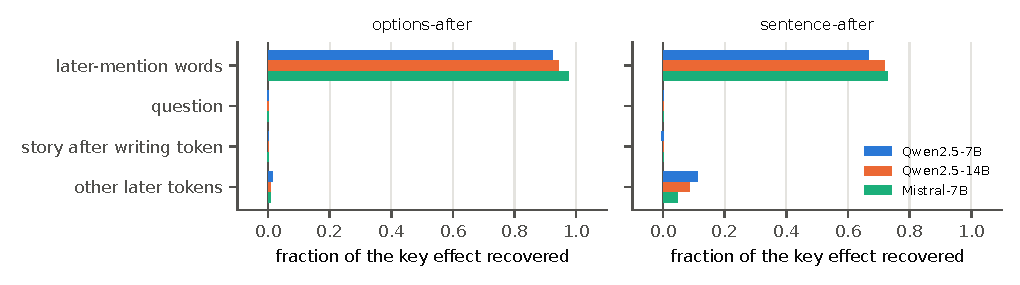
\includegraphics[width=0.85\textwidth]{figures/fig_localisation.pdf}
\caption{\textbf{Which later tokens read the writing token's key} (discovery sample; preregistration D, D3). Fraction of the full key effect recovered when only one group of later tokens sees the source key, at Qwen2.5-7B, Qwen2.5-14B and Mistral-7B, under \fmtOpt{} and \fmtPost{}; $n = 60$ stories; values with intervals in \cref{tab:localisation}.}
\label{fig:localisation}
\end{figure}

\paragraph{Attention probe.} An early exploratory probe at Qwen2.5-1.5B ($n = 25$ cores, no CIs, a different prompt) found that the option word naming the source location attends to the writing token as in the source run when the writing token's key is swapped. Part (a) of preregistration G supersedes it (\cref{app:g-attention}).

\paragraph{Preregistration G.} Preregistration G (GPU stage 5) asked what the duplicate-token account predicts and where it stops. Parts (a)--(d) use the 150 seed-0 story cores of stages 1 and 3b (the row splice and the form probe the first 60 of them), and part (e) 200 fresh IOI cores. Every contrast is paired by core, with 95\% percentile intervals from 10{,}000 core-bootstrap resamples and ratios of means recomputed within each resample. \Cref{tab:prereg-g} gives every verdict; here we define the measures, give the per-cell values and report the observations that the entry did not predict, without reinterpreting them. A shared gate required the stage-5 factorial to reproduce the stage-3b $\mathrm{ID}_K$ of \fmtPost{}, \fmtNone{} and \fmtListA{} in the four models of parts (c) and (d); every value agrees at the printed precision. Triples are Qwen2.5-7B / Qwen2.5-14B / Mistral-7B unless stated.

\subsubsection{(a) Re-mention attention at every scale}\label{app:g-attention}

Under \fmtPost{} the neutral sentence mentions the written word B again. With eager attention, we take for each head the attention from that mention to the writing token, minus the mean attention to the writing token from the candidates not mentioned before it. The three heads with the largest mean excess on the odd-indexed cores form $H^*$. On the even-indexed cores, $E$ is the mean excess at $H^*$, and $F$ is the gain in the attention from the mention of S to the writing token under the key clamp $\mathcal{C}_K(\mathrm{S})$, so $F/E = 1$ means that the attention follows the clamped key one for one. $G$ is the same excess for the answer position's attention to the mention of B (hop~2), at its own three heads, and $Q$ is $G$ at a small model divided by the smaller $G$ of the two anchors, Qwen2.5-7B and 14B. \Cref{tab:attention} gives every cell.

\begin{table}[!ht]
\centering
\small
\caption{\textbf{Re-mention attention} (preregistration G, part (a)). $E$: excess attention of the later mention of B to the writing token at the three selected heads; $F/E$: the share of it that follows the key clamp; $G$: excess attention of the answer position to the mention of B (hop~2) at its own three heads; $\mathrm{ID}_K$ and the non-specific key effect $d_K$ (nats) from the same eager run, scored in the casing the model emits. Heads selected on odd-indexed and evaluated on even-indexed cores of 150; 95\% bootstrap CIs. Under \fmtPost{}: G1 at 7B and 14B, G2 and G3 at 1.5B and 3B, G4 in all four; \fmtOpt{} is the gate and the reference of G3.}
\label{tab:attention}
\begin{tabular}{@{}llccccc@{}}
\toprule
Model & Format & $E$ & $F/E$ & $G$ (hop 2) & $\mathrm{ID}_K$ (nats) & $d_K$ (nats) \\
\midrule
Qwen2.5-1.5B & \fmtPost{} & \begin{tabular}[t]{@{}c@{}}0.789\\[-1pt]{\scriptsize[0.778, 0.802]}\end{tabular} & 1.03 & \begin{tabular}[t]{@{}c@{}}0.086\\[-1pt]{\scriptsize[0.075, 0.098]}\end{tabular} & \begin{tabular}[t]{@{}c@{}}$-$0.53\\[-1pt]{\scriptsize[$-$0.64, $-$0.41]}\end{tabular} & $+$0.31 \\
 & \fmtOpt{} & \begin{tabular}[t]{@{}c@{}}0.750\\[-1pt]{\scriptsize[0.734, 0.767]}\end{tabular} & 1.04 & \begin{tabular}[t]{@{}c@{}}0.453\\[-1pt]{\scriptsize[0.423, 0.484]}\end{tabular} & \begin{tabular}[t]{@{}c@{}}$+$2.63\\[-1pt]{\scriptsize[2.41, 2.86]}\end{tabular} & $+$5.96 \\
\midrule
Qwen2.5-3B & \fmtPost{} & \begin{tabular}[t]{@{}c@{}}0.879\\[-1pt]{\scriptsize[0.866, 0.892]}\end{tabular} & 0.99 & \begin{tabular}[t]{@{}c@{}}0.113\\[-1pt]{\scriptsize[0.095, 0.132]}\end{tabular} & \begin{tabular}[t]{@{}c@{}}$+$0.04\\[-1pt]{\scriptsize[$-$0.35, 0.44]}\end{tabular} & $+$3.03 \\
 & \fmtOpt{} & \begin{tabular}[t]{@{}c@{}}0.832\\[-1pt]{\scriptsize[0.821, 0.844]}\end{tabular} & 1.03 & \begin{tabular}[t]{@{}c@{}}0.395\\[-1pt]{\scriptsize[0.355, 0.435]}\end{tabular} & \begin{tabular}[t]{@{}c@{}}$+$10.37\\[-1pt]{\scriptsize[9.62, 11.13]}\end{tabular} & $+$20.57 \\
\midrule
Qwen2.5-7B & \fmtPost{} & \begin{tabular}[t]{@{}c@{}}0.869\\[-1pt]{\scriptsize[0.852, 0.885]}\end{tabular} & 1.00 & \begin{tabular}[t]{@{}c@{}}0.255\\[-1pt]{\scriptsize[0.222, 0.288]}\end{tabular} & \begin{tabular}[t]{@{}c@{}}$+$4.73\\[-1pt]{\scriptsize[4.39, 5.07]}\end{tabular} & $+$9.21 \\
 & \fmtOpt{} & \begin{tabular}[t]{@{}c@{}}0.887\\[-1pt]{\scriptsize[0.874, 0.900]}\end{tabular} & 1.00 & \begin{tabular}[t]{@{}c@{}}0.770\\[-1pt]{\scriptsize[0.739, 0.798]}\end{tabular} & \begin{tabular}[t]{@{}c@{}}$+$19.39\\[-1pt]{\scriptsize[19.00, 19.78]}\end{tabular} & $+$36.90 \\
\midrule
Qwen2.5-14B & \fmtPost{} & \begin{tabular}[t]{@{}c@{}}0.915\\[-1pt]{\scriptsize[0.908, 0.921]}\end{tabular} & 0.98 & \begin{tabular}[t]{@{}c@{}}0.329\\[-1pt]{\scriptsize[0.304, 0.353]}\end{tabular} & \begin{tabular}[t]{@{}c@{}}$+$13.48\\[-1pt]{\scriptsize[12.76, 14.20]}\end{tabular} & $+$24.09 \\
 & \fmtOpt{} & \begin{tabular}[t]{@{}c@{}}0.866\\[-1pt]{\scriptsize[0.856, 0.876]}\end{tabular} & 0.99 & \begin{tabular}[t]{@{}c@{}}0.865\\[-1pt]{\scriptsize[0.859, 0.872]}\end{tabular} & \begin{tabular}[t]{@{}c@{}}$+$38.95\\[-1pt]{\scriptsize[37.88, 39.97]}\end{tabular} & $+$74.79 \\
\bottomrule
\end{tabular}

\end{table}

At 1.5B and 3B the re-mention attends to the writing token about as strongly as at 7B and 14B, and the attention follows the clamped key, while $\mathrm{ID}_K$ under \fmtPost{} stays within the preregistered $\pm 1$-nat margin (G2, $H_{\mathrm{diss}}$; G3). By the entry's criterion the heads are not embedding-level, and the same heads serve both formats at 1.5B and 7B (overlap of the two $H^*$, as a Jaccard index, \GaJaccardQwenOnefive{} and \GaJaccardQwenSeven{}; \GaJaccardQwenThree{} at 3B). Hop-2 attention is weaker at the small models ($Q$ = \GfourbQQwenOnefive{} and \GfourbQQwenThree{}; G4), but at 3B it reaches the presence bar that G4a sets for the anchors without any key read, so it does not alone account for the scale difference. $G$ measures attention; it does not intervene on hop~2.

\emph{Unpredicted observations.} (i)~At 3B the key clamp has a non-specific effect without identity ($d_K$ = \GaDKCapPostQwenThree{} nats against $\mathrm{ID}_K$ = \GaIDKCapPostQwenThree{}). (ii)~Under \fmtPost{} only \GaCompetentPostQwenOnefive{} and \GaCompetentPostQwenThree{} of the cores at the small models are answered correctly in both clean runs, and almost every wrong answer is the initial location; on the competent cores the 3B value is slightly positive, as in the stage-1 competent-only analysis (\cref{app:additional}; recomputed, not preregistered). (iii)~Under the key clamp, the answer's hop-2 attention does not follow the clamped key at 1.5B (change towards the mention of S \GaDansSPostQwenOnefive{}, towards B \GaDansBPostQwenOnefive{}), partly follows it at 3B (\GaDansSPostQwenThree{} and $\GaDansBPostQwenThree$) and follows it at 7B and 14B (\GaDansSPostQwenSeven{} and $\GaDansBPostQwenSeven$; \GaDansSPostQwenFourteen{} and $\GaDansBPostQwenFourteen$). (iv)~Under \fmtPost{} at 7B and 14B, the answer row at the hop-2 heads attends mostly to the writing token itself (\GaAnsToPQwenSeven{} and \GaAnsToPQwenFourteen{}), not to the re-mentions; under \fmtOpt{} its five largest columns are all re-mentioned words. (v)~The two formats' $H^*$ overlap little at 14B (\GaJaccardQwenFourteen{}), but each format's heads still work on the other (cross-format $E$ = \GaEcrossPostQwenFourteen{} and \GaEcrossOptQwenFourteen{}).

\subsubsection{(b) Attention knockout}\label{app:g-knockout}

A knockout sets the attention from a set of rows to a set of columns to zero in every layer and head (\cref{app:impl}). The preregistered masks are M0, none; M1, the six candidate words after the writing token to the writing token; M2, the same rows to the earlier occurrences of the initial-location word, a matched control column; M3, the answer position to the writing token; M4, the union of M1 and M3; and M8, every later row to the writing token, a sanity gate. The exploratory masks are M2b, the candidate rows to the token before the writing token; M5, only the rows of the three clamped candidates B, S and X; M6, the other three candidate rows; M7, every later row that is not a candidate word; Mq, the question rows; and Mpost, the rows between the candidates and the answer position. $r_K$ is $\mathrm{ID}_K$ under the mask divided by $\mathrm{ID}_K$ without it; $q_V = \mathrm{ID}_V/d_{KV}$ is the value identity as a share of the joint clamp's effect; acc$_B$ is the fraction of cores whose answer, restricted to the candidates, is still B. \Cref{tab:knockout} gives every cell.

\begin{table}[!ht]
\centering
\small
\caption{\textbf{Attention knockout} (preregistration G, part (b); masks in the text). $r_K$: $\mathrm{ID}_K$ under the mask relative to no mask; $q_V$: $\mathrm{ID}_V$ as a share of the joint clamp's effect $d_{KV}$; acc$_B$: fraction of cores whose candidate-restricted answer is B. $n = 150$ cores per cell. M1, M2, M3, M4 and M8 enter G5--G8 and Gate b; the other masks, and every mask under \fmtPost{}, are exploratory. Under \fmtNone{} only the masks that do not need candidate rows are defined.}
\label{tab:knockout}
\begin{tabular}{@{}llccccccccc@{}}
\toprule
Format & Mask & \multicolumn{3}{c}{Qwen2.5-7B} & \multicolumn{3}{c}{Qwen2.5-14B} & \multicolumn{3}{c}{Mistral-7B} \\
\cmidrule(lr){3-5}\cmidrule(lr){6-8}\cmidrule(lr){9-11}
 & & $r_K$ & $q_V$ & acc$_B$ & $r_K$ & $q_V$ & acc$_B$ & $r_K$ & $q_V$ & acc$_B$ \\
\midrule
\fmtListA{} & M0 & 1.000 & 0.125 & 1.00 & 1.000 & 0.075 & 1.00 & 1.000 & 0.105 & 1.00 \\
 & M1 & 0.001 & 0.390 & 0.37 & $-$0.026 & 0.440 & 1.00 & $-$0.007 & 0.448 & 0.86 \\
 & M2 & 1.094 & 0.104 & 1.00 & 0.997 & 0.065 & 1.00 & 0.990 & 0.113 & 1.00 \\
 & M2b & 1.001 & 0.125 & 1.00 & 1.000 & 0.075 & 1.00 & 1.000 & 0.107 & 1.00 \\
 & M3 & 1.043 & 0.022 & 1.00 & 1.027 & 0.017 & 1.00 & 1.010 & 0.053 & 1.00 \\
 & M4 & 0.001 & 0.512 & 0.00 & 0.001 & 0.470 & 0.66 & $-$0.001 & 0.457 & 0.39 \\
 & M5 & $-$0.008 & 0.418 & 0.73 & $-$0.025 & 0.446 & 1.00 & $-$0.007 & 0.457 & 0.89 \\
 & M6 & 0.961 & 0.117 & 1.00 & 1.003 & 0.071 & 1.00 & 1.003 & 0.106 & 1.00 \\
 & M7 & 0.947 & 0.003 & 0.97 & 1.022 & 0.004 & 1.00 & 0.948 & 0.020 & 0.97 \\
 & M8 & 0.000 & -- & 0.00 & 0.000 & -- & 0.13 & 0.000 & -- & 0.17 \\
 & Mq & 0.981 & 0.123 & 1.00 & 1.002 & 0.076 & 1.00 & 0.988 & 0.112 & 1.00 \\
 & Mpost & 1.001 & 0.119 & 1.00 & 1.002 & 0.068 & 1.00 & 0.999 & 0.096 & 1.00 \\
\midrule
\fmtOpt{} & M0 & 1.000 & 0.120 & 1.00 & 1.000 & 0.066 & 1.00 & 1.000 & 0.074 & 1.00 \\
 & M1 & 0.003 & 0.377 & 0.30 & $-$0.028 & 0.427 & 0.99 & $-$0.009 & 0.422 & 0.73 \\
 & M2 & 1.071 & 0.099 & 1.00 & 0.998 & 0.057 & 1.00 & 0.972 & 0.083 & 1.00 \\
 & M2b & 1.000 & 0.120 & 1.00 & 0.999 & 0.066 & 1.00 & 1.001 & 0.077 & 1.00 \\
 & M3 & 1.041 & 0.019 & 1.00 & 1.017 & 0.013 & 1.00 & 1.006 & 0.040 & 1.00 \\
 & M4 & 0.000 & 0.523 & 0.00 & 0.002 & 0.464 & 0.58 & 0.001 & 0.446 & 0.29 \\
 & M5 & $-$0.004 & 0.404 & 0.58 & $-$0.027 & 0.435 & 1.00 & $-$0.008 & 0.429 & 0.77 \\
 & M6 & 0.971 & 0.113 & 1.00 & 1.005 & 0.059 & 1.00 & 1.007 & 0.077 & 1.00 \\
 & M7 & 0.944 & 0.001 & 0.98 & 0.983 & 0.004 & 1.00 & 0.926 & 0.015 & 0.99 \\
 & M8 & 0.000 & -- & 0.00 & 0.000 & -- & 0.10 & 0.000 & -- & 0.19 \\
 & Mq & 0.980 & 0.119 & 1.00 & 0.997 & 0.068 & 1.00 & 0.993 & 0.079 & 1.00 \\
 & Mpost & 1.001 & 0.118 & 1.00 & 0.998 & 0.065 & 1.00 & 1.000 & 0.070 & 1.00 \\
\midrule
\fmtPost{} & M0 & 1.000 & 0.346 & 1.00 & 1.000 & 0.325 & 1.00 & 1.000 & 0.361 & 1.00 \\
 & M1 & $-$0.105 & 0.423 & 1.00 & $-$0.036 & 0.443 & 1.00 & 0.001 & 0.460 & 0.99 \\
 & M2 & 1.027 & 0.346 & 1.00 & 0.922 & 0.333 & 1.00 & 0.963 & 0.368 & 1.00 \\
 & M2b & 1.007 & 0.346 & 1.00 & 0.994 & 0.327 & 1.00 & 0.991 & 0.362 & 1.00 \\
 & M3 & 1.660 & 0.099 & 0.77 & 1.800 & 0.117 & 1.00 & 1.394 & 0.188 & 0.99 \\
 & M4 & 0.007 & 0.496 & 0.07 & 0.014 & 0.480 & 0.91 & 0.002 & 0.446 & 0.29 \\
 & M5 & $-$0.113 & 0.423 & 1.00 & $-$0.035 & 0.443 & 1.00 & $-$0.003 & 0.464 & 1.00 \\
 & M6 & 0.974 & 0.348 & 1.00 & 1.053 & 0.319 & 1.00 & 0.995 & 0.359 & 1.00 \\
 & M7 & 1.184 & $-$0.036 & 0.35 & 1.939 & $-$0.016 & 1.00 & 1.456 & 0.012 & 0.86 \\
 & M8 & 0.000 & -- & 0.00 & 0.000 & -- & 0.14 & 0.000 & -- & 0.05 \\
 & Mq & 0.929 & 0.349 & 0.99 & 1.005 & 0.323 & 1.00 & 1.000 & 0.359 & 1.00 \\
 & Mpost & 1.028 & 0.329 & 0.99 & 1.327 & 0.255 & 1.00 & 1.209 & 0.290 & 1.00 \\
\midrule
\fmtNone{} & M0 & 1.000 & 0.391 & 1.00 & 1.000 & 0.335 & 1.00 & 1.000 & 0.433 & 1.00 \\
 & M3 & 0.023 & 0.566 & 0.00 & 0.041 & 0.459 & 0.20 & 0.117 & 0.445 & 0.15 \\
 & M8 & 0.000 & -- & 0.00 & 0.000 & -- & 0.00 & 0.000 & -- & 0.12 \\
 & Mq & 0.967 & 0.388 & 1.00 & 1.005 & 0.331 & 1.00 & 0.988 & 0.432 & 1.00 \\
 & Mpost & 1.040 & 0.378 & 1.00 & 1.004 & 0.318 & 1.00 & 0.995 & 0.402 & 1.00 \\
\bottomrule
\end{tabular}

\end{table}

Cutting the candidate words' attention to the writing token removes the key read in every format and model, the control column does not, and cutting the answer's own attention leaves the read intact (G5, G6, G8b). The copy returns to its \fmtNone{} share on the identity measure (G7a), but the answer is kept only at Qwen2.5-14B (G7b): the preregistered outcome is a partial takeover. Under \fmtNone{}, M3 leaves \GeightaRatioQwenSeven{} / \GeightaRatioQwenFourteen{} / \GeightaRatioMistralSeven{} of $\mathrm{ID}_V$ (G8a), but it also removes most of the writing token's whole effect and of the models' ability to answer (\cref{tab:knockout}).

\emph{Unpredicted observations.} (i)~At Qwen2.5-7B, the answer that replaces B under M1 is mostly the initial location (exploratory, recomputed, descriptive); G7b's location-mass criterion cannot see these answers, because they are location words too. (ii)~Under \fmtPost{}, cutting only the answer's attention to the writing token (M3) raises the key read ($r_K$ = \GbRKPostMthreeQwenSeven{} / \GbRKPostMthreeQwenFourteen{} / \GbRKPostMthreeMistralSeven{}), and so does M7. (iii)~Cutting only the rows of the three clamped candidates (M5) removes the read as completely as M1 (under \fmtListA{}, $r_K$ = $\GbRKAfterMfiveQwenSeven$ / $\GbRKAfterMfiveQwenFourteen$ / $\GbRKAfterMfiveMistralSeven$), while cutting the other three (M6) leaves it intact (\GbRKAfterMsixQwenSeven{} / \GbRKAfterMsixQwenFourteen{} / \GbRKAfterMsixMistralSeven{}). (iv)~Under \fmtPost{}, M1 raises $q_V$ to \GbQVPostMoneQwenSeven{} / \GbQVPostMoneQwenFourteen{} / \GbQVPostMoneMistralSeven{}. (v)~At Qwen2.5-7B, cutting the control column (M2) slightly strengthens the key read ($r_K$ = \GsixRKQwenSeven{}).

\subsubsection{(c) Membership and dose}\label{app:g-membership}

The arms replace the neutral sentence (family S) or the option list (family L) by one that names a subset of the candidates, in the canonical order and with ``Answer with one word'': S2 and L2 name S and X; S3 and L3 name B, S and X; S3out and L3out name B and two candidates other than S and X; S3half names B, S and one other; S4 and L4 name B, S, X and one other; S4out and L4out name S, X and two others, but not B; and S6 and L6 are \fmtPost{} and \fmtListA{}. $r_k$ is $\mathrm{ID}_K$ in the arm naming $k$ candidates divided by $\mathrm{ID}_K$ in the arm naming all six. The row splice (first 60 cores) lets only the named words' rows see the source key, giving $f_{\mathrm{words}}$, their share of the total splice effect $d$. \Cref{tab:membership} gives every arm.

\begin{table}[!ht]
\centering
\small
\caption{\textbf{Membership and dose} (preregistration G, part (c)). Top: $\mathrm{ID}_K$ and $\mathrm{ID}_V$ (nats) per arm, seed-0 cores, $n = 150$. Bottom: row splice ($n = 60$), the share of the total key-swap effect $d$ read by the named words' rows ($f_{\mathrm{words}}$) and by the rows after the question. Qwen2.5-7B, Qwen2.5-14B and Mistral-7B enter G9--G12; OLMo-2-7B and the arms S3half, S4, S4out, L4, L4out, S6, L6 (as splice arms) and S3out, L3out (as splice arms) are exploratory.}
\label{tab:membership}
\begin{tabular}{@{}lcccccccc@{}}
\toprule
Arm & \multicolumn{2}{c}{Qwen2.5-7B} & \multicolumn{2}{c}{Qwen2.5-14B} & \multicolumn{2}{c}{Mistral-7B} & \multicolumn{2}{c}{OLMo-2-7B} \\
\cmidrule(lr){2-3}\cmidrule(lr){4-5}\cmidrule(lr){6-7}\cmidrule(lr){8-9}
 & $\mathrm{ID}_K$ & $\mathrm{ID}_V$ & $\mathrm{ID}_K$ & $\mathrm{ID}_V$ & $\mathrm{ID}_K$ & $\mathrm{ID}_V$ & $\mathrm{ID}_K$ & $\mathrm{ID}_V$ \\
\midrule
\fmtNone{} & $+$1.04 & $+$16.60 & $+$1.05 & $+$19.12 & $+$0.55 & $+$13.65 & $+$0.38 & $+$10.97 \\
S2 & $+$1.52 & $+$13.97 & $+$6.99 & $+$23.51 & $+$3.66 & $+$13.22 & $+$0.86 & $+$8.55 \\
S3 & $+$3.49 & $+$11.94 & $+$9.52 & $+$19.67 & $+$5.25 & $+$11.83 & $+$1.51 & $+$8.75 \\
S3half & $+$2.11 & $+$12.13 & $+$5.41 & $+$16.16 & $+$2.66 & $+$11.79 & $+$0.67 & $+$8.37 \\
S3out & $+$0.73 & $+$12.61 & $+$0.75 & $+$13.40 & $+$0.34 & $+$12.18 & $+$0.29 & $+$8.84 \\
S4 & $+$4.59 & $+$12.26 & $+$10.88 & $+$18.88 & $+$6.15 & $+$11.87 & $+$1.64 & $+$8.69 \\
S4out & $+$4.18 & $+$14.08 & $+$10.82 & $+$24.36 & $+$6.17 & $+$13.58 & $+$1.59 & $+$8.96 \\
S6 & $+$5.52 & $+$11.91 & $+$12.08 & $+$18.46 & $+$7.87 & $+$11.46 & $+$2.01 & $+$8.63 \\
\midrule
L2 & $+$19.76 & $+$18.63 & $+$35.19 & $+$29.48 & $+$15.27 & $+$16.24 & $+$5.87 & $+$10.03 \\
L3 & $+$21.70 & $+$4.06 & $+$35.83 & $+$2.97 & $+$15.66 & $+$3.29 & $+$7.89 & $+$5.14 \\
L3out & $+$0.69 & $+$5.49 & $+$0.92 & $+$3.49 & $+$0.31 & $+$2.47 & $+$0.37 & $+$4.30 \\
L4 & $+$21.50 & $+$4.71 & $+$35.87 & $+$4.19 & $+$15.38 & $+$3.62 & $+$8.35 & $+$5.33 \\
L4out & $+$20.29 & $+$14.90 & $+$35.45 & $+$30.76 & $+$15.45 & $+$13.68 & $+$8.00 & $+$9.07 \\
L6 & $+$20.60 & $+$5.93 & $+$35.81 & $+$5.69 & $+$15.55 & $+$3.44 & $+$8.65 & $+$5.93 \\
\midrule
\multicolumn{9}{@{}l}{\emph{Reader rows (splice, $n = 60$): $f_{\mathrm{words}}$ / share read by the rows after the question}} \\
S2 & \multicolumn{2}{c}{0.40 / 0.46} & \multicolumn{2}{c}{0.38 / 0.49} & \multicolumn{2}{c}{0.39 / 0.38} & \multicolumn{2}{c}{0.26 / 0.62} \\
S3 & \multicolumn{2}{c}{0.68 / 0.13} & \multicolumn{2}{c}{0.72 / 0.11} & \multicolumn{2}{c}{0.72 / 0.10} & \multicolumn{2}{c}{0.90 / $-$0.01} \\
S6 & \multicolumn{2}{c}{0.67 / 0.11} & \multicolumn{2}{c}{0.72 / 0.09} & \multicolumn{2}{c}{0.73 / 0.05} & \multicolumn{2}{c}{0.76 / 0.06} \\
S3out & \multicolumn{2}{c}{0.04 / 0.90} & \multicolumn{2}{c}{0.11 / 0.74} & \multicolumn{2}{c}{0.11 / 0.68} & \multicolumn{2}{c}{$-$0.16 / 1.40} \\
L2 & \multicolumn{2}{c}{0.91 / 0.14} & \multicolumn{2}{c}{0.94 / 0.17} & \multicolumn{2}{c}{0.92 / 0.08} & \multicolumn{2}{c}{0.72 / 0.13} \\
L3 & \multicolumn{2}{c}{0.94 / 0.01} & \multicolumn{2}{c}{0.95 / 0.00} & \multicolumn{2}{c}{0.95 / 0.01} & \multicolumn{2}{c}{0.91 / $-$0.01} \\
L6 & \multicolumn{2}{c}{0.91 / 0.01} & \multicolumn{2}{c}{0.93 / 0.01} & \multicolumn{2}{c}{0.95 / 0.01} & \multicolumn{2}{c}{0.88 / 0.00} \\
L3out & \multicolumn{2}{c}{0.58 / 0.13} & \multicolumn{2}{c}{0.39 / 0.09} & \multicolumn{2}{c}{0.41 / 0.18} & \multicolumn{2}{c}{0.58 / 0.31} \\
\bottomrule
\end{tabular}

\end{table}

The key read needs the swapped candidates themselves: naming B with two others gives none (G9, met in both families and replicated at seed~1). In lists two named candidates give the full read; in sentences the read grows with the number named, and at Qwen2.5-7B $r_2$ = \GtenSRtwoQwenSeven{} (\GtenSRtwoSeedoneQwenSeven{} at seed~1) is not above proportional (G10, met for lists, not for sentences). Removing S and X from a list does not bring the copy back ($R_V$ = \GelevenRVQwenSeven{} / \GelevenRVQwenFourteen{} / $\GelevenRVMistralSeven$; G11, not met). In a sentence naming only S and X (S2), the named words carry \GtwelveStwoQwenSeven{} / \GtwelveStwoQwenFourteen{} / \GtwelveStwoMistralSeven{} of the splice effect and the rows after the question \GtwelveRestStwoQwenSeven{} / \GtwelveRestStwoQwenFourteen{} / \GtwelveRestStwoMistralSeven{} (G12, not met, 9/12). G12 splits the total key-swap effect $d$, not $\mathrm{ID}_K$, and in S2 most of $d$ is not identity-specific: $\mathrm{ID}_K/d_K$ is \GcShareStwoQwenSeven{} / \GcShareStwoQwenFourteen{} / \GcShareStwoMistralSeven{} in S2 against \GcShareSthreeQwenSeven{} / \GcShareSthreeQwenFourteen{} / \GcShareSthreeMistralSeven{} in S3 (arithmetic on printed values). The main text's narrowing to ``lists and sentences naming at least three candidates'' rests on this.

\emph{Unpredicted observations.} (i)~Naming B with two other candidates pushes $\mathrm{ID}_K$ below \fmtNone{}, although the written word is re-mentioned (S3out$-$\fmtNone{} $\GnineSOutNoneQwenSeven$, L3out$-$\fmtNone{} $\GnineLOutNoneQwenSeven$ at Qwen2.5-7B; \cref{tab:prereg-g}). (ii)~In sentences every added candidate raises $\mathrm{ID}_K$: at Qwen2.5-7B the paired steps are S3$-$S2 = \GtenSStepThreeTwoQwenSeven{} (adds B), S4$-$S3 = \GtenSStepFourThreeQwenSeven{} (adds one non-matching candidate) and S6$-$S4 = \GtenSStepSixFourQwenSeven{} (adds two), each with a CI excluding zero; a pure duplicate-token account does not predict the last two. Naming one of the two swapped candidates (S3half) gives about half of S3 (\GcHalfQwenSeven{} at Qwen2.5-7B). (iii)~In lists that do not name the written word B, the key read is at full strength while the value identity stays near or above \fmtNone{}: $\mathrm{ID}_V$(L4out) is \GcIDVLfouroutQwenSeven{} / \GcIDVLfouroutQwenFourteen{} / \GcIDVLfouroutMistralSeven{} against \GcIDVNoneQwenSeven{} / \GcIDVNoneQwenFourteen{} / \GcIDVNoneMistralSeven{} under \fmtNone{} and \GcIDVLthreeQwenSeven{} / \GcIDVLthreeQwenFourteen{} / \GcIDVLthreeMistralSeven{} in L3. This suggests, post hoc, that the copy is suppressed when the written word itself is re-mentioned; it is a hypothesis for a future test, not a claim. (iv)~Under \fmtNone{} and every sentence arm, the clean answer puts almost no probability on the six lowercase candidates at the three primary models, so the sentence-family contrasts are scored on tokens the model is not about to emit, as in stage 3b; in lists the candidates carry most of it.

\subsubsection{(d) Non-identical re-mentions}\label{app:g-forms}

Each variant replaces the re-mentions of the \fmtPost{} sentence: THE adds ``the''; MODIF uses a modified noun phrase (``wooden shelf''); TITLE and UPPER change the case; PLURAL uses the plural; SYN a synonym; FRMIX and DEMIX put the French or German word in the English frame; FR and DE translate the whole sentence (exploratory); and three structure-matched floor sentences name other words. With the floor and the exact repeat (\fmtPost{}) scored on the English candidates, $r_K(v) = [\mathrm{ID}_K(v) - \mathrm{ID}_K(\text{floor})]/[\mathrm{ID}_K(\text{\fmtPost{}}) - \mathrm{ID}_K(\text{floor})]$; $r_K^{\mathrm{any}}$ also scores the answer in the variant's own form; $\rho_s$ is the ratio of the identity key shares; and $a_v$ is the variant's attention to the writing token, summed over its tokens, relative to the exact repeat's ($n = 60$). Gates required clean accuracy of at least 0.95 in the variant, its floor and its anchor, and that at least five of the six words map correctly in a six-way prompt (the passing words are the population of the cell). A prediction is met if at least three evaluable models meet it. \Cref{tab:variants} gives every cell.

\begin{table}[!ht]
\centering
\caption{\textbf{Non-identical re-mentions} (preregistration G, part (d)). $r_K$: key identity relative to an exact repeat, above a structure-matched floor, on the English candidates; $r_K^{\mathrm{any}}$: the same with the answer also scored in the variant's own form; $a_v$: attention of the re-mention to the writing token relative to the exact repeat, summed over the re-mention's tokens ($n = 60$). $n = 150$ cores per cell before the per-word competence gate; DEMIX and DE cover fewer cores. THE, MODIF, TITLE, UPPER, PLURAL, SYN, FRMIX and DEMIX enter G13--G16; FR, DE and the list variant are exploratory.}
\label{tab:variants}
\resizebox{\textwidth}{!}{\begin{tabular}{@{}lcccccccccccc@{}}
\toprule
Variant & \multicolumn{3}{c}{Qwen2.5-7B} & \multicolumn{3}{c}{Qwen2.5-14B} & \multicolumn{3}{c}{Mistral-7B} & \multicolumn{3}{c}{OLMo-2-7B} \\
\cmidrule(lr){2-4}\cmidrule(lr){5-7}\cmidrule(lr){8-10}\cmidrule(lr){11-13}
 & $r_K$ & $r_K^{\mathrm{any}}$ & $a_v$ & $r_K$ & $r_K^{\mathrm{any}}$ & $a_v$ & $r_K$ & $r_K^{\mathrm{any}}$ & $a_v$ & $r_K$ & $r_K^{\mathrm{any}}$ & $a_v$ \\
\midrule
THE & 1.09 & 1.09 & 1.09 & 0.99 & 0.99 & 1.02 & 1.06 & 1.06 & 1.11 & 0.96 & 0.96 & 1.02 \\
MODIF & 0.32 & 0.32 & 1.22 & 0.64 & 0.64 & 1.24 & 0.64 & 0.64 & 1.08 & 0.55 & 0.55 & 0.94 \\
TITLE & 0.94 & 1.19 & 0.92 & 1.09 & 1.37 & 0.97 & 1.07 & 1.53 & 1.79 & 0.87 & 0.89 & 0.90 \\
UPPER & 1.08 & 1.51 & 1.74 & 1.14 & 1.57 & 1.93 & 1.01 & 1.26 & 2.58 & 0.83 & 0.90 & 1.84 \\
PLURAL & 0.33 & 0.33 & 0.87 & 0.37 & 0.37 & 0.88 & 0.49 & 0.50 & 1.40 & 0.11 & 0.11 & 0.89 \\
SYN & $-$0.03 & 0.09 & 0.41 & 0.00 & 0.09 & 0.41 & 0.06 & 0.26 & 0.53 & $-$0.13 & $-$0.13 & 0.21 \\
FRMIX & 0.15 & 0.95 & 0.86 & 0.10 & 1.06 & 0.90 & 0.07 & 0.56 & 0.55 & 0.09 & 0.44 & 0.39 \\
DEMIX & $-$0.01 & 0.69 & 0.66 & 0.02 & 1.32 & 0.65 & 0.02 & 0.31 & 0.33 & 0.00 & $-$0.13 & 0.09 \\
FR & 0.18 & 0.55 & 1.16 & 0.18 & 0.47 & 1.21 & 0.14 & 0.28 & 0.83 & 0.16 & 0.41 & 0.58 \\
DE & 0.00 & 0.59 & 0.92 & 0.06 & 1.06 & 1.01 & 0.05 & 0.55 & 0.58 & $-$0.05 & 0.43 & 0.30 \\
list SYN & 0.05 & 0.33 & -- & 0.05 & 0.23 & -- & 0.07 & 0.47 & -- & 0.00 & 0.05 & -- \\
\bottomrule
\end{tabular}
}
\end{table}

On our English-scored measure the read is bound to the word form (G15): synonyms and mixed-language words carry at most \GfifteenRKMax{} of an exact repeat's key identity. It is largely insensitive to case (TITLE and UPPER read \GfourteenCaseMin{}--\GfourteenCaseMax{}; G14 not met for them), sensitive to number (PLURAL \GfourteenPluralMin{}--\GfourteenPluralMax{}), and a modified noun phrase reads only partly (MODIF \GthirteenModifMin{}--\GthirteenModifMax{}; G13 not met for it, THE met). No preregistered token-or-concept outcome holds for any variant (G16, not met): the profile is graded and model-dependent. Per model, and exploratory: at the two Qwen models FRMIX shows the concept pattern on both measures ($r_K^{\mathrm{any}}$ = \GdRKanyFrmixQwenSeven{} and \GdRKanyFrmixQwenFourteen{}; $a_v$ = \GdAvFrmixQwenSeven{} and \GdAvFrmixQwenFourteen{}), and scored in its own form it reads fully ($r_K$ = \GdRKformFrmixQwenSeven{} and \GdRKformFrmixQwenFourteen{}); DEMIX is concept-like on $r_K^{\mathrm{any}}$ but graded on $a_v$ there; at Mistral-7B and OLMo-2-7B the read is graded or token-level. Where the read is lost, the value identity rises (G17, met), but by no more than after the floor sentence that names other words (exploratory: the floor sentence raises $\mathrm{ID}_V$ over \fmtPost{} by \GdOtherCompQwenSeven{}, \GdOtherCompMistralSeven{} and \GdOtherCompOlmoSeven{} nats at Qwen2.5-7B, Mistral-7B and OLMo-2-7B, recomputed, against \GseventeenFrmixQwenSeven{}, \GseventeenFrmixMistralSeven{} and \GseventeenFrmixOlmoSeven{} for FRMIX).

\emph{Unpredicted observations.} (i)~A capitalised or upper-case re-mention reads nearly as fully as the exact repeat, although its token ids differ; the CI lies below 1 in three of the eight cells. (ii)~MODIF attends to the writing token about as much as the exact repeat ($a_v$ = \GdAvModifQwenSeven{}, \GdAvModifQwenFourteen{}, \GdAvModifMistralSeven{} and \GdAvModifOlmoSeven{} in the four models) but reads the key only partly: attention without the read. Values of $a_v$ above 1 come from summing attention over multi-token spans; with the last token only, the FRMIX attention leg falls below the concept bar (exploratory, recomputed in the log). (iii)~The raw rise of $\log p(\mathrm{S})$ under the key clamp does not separate the variants, so only the identity contrasts are reported.

\subsection{Reader heads and the second hop}\label{app:heads}\label{sec:heads}\label{sec:role}\label{app:stage6}

Preregistration H (GPU stage 6) has two parts: the heads that read the writing token's key and the route from them to the answer, at two 7B models (this subsection), and the key-only and value-only exchange applied to the binding intervention of \citet{prakash2025lookbacks} at Qwen2.5-14B (\cref{app:prakash}). \Cref{tab:prereg-h} gives every gate and verdict, and \cref{app:prereg-ai} the disclosures.

\paragraph{Summary (discovery sample).} Preregistration H looked inside the option rows at Qwen2.5-7B and Mistral-7B under \fmtOpt{} (\cref{tab:heads}); H1--H5 were met in both. When only the top 5\% of heads by $a_3$ (\HkstarQwenSeven{} and \HkstarMistralSeven{}) see the source key, they recover $R(k^*) = \HoneRQwenSeven{}$ and \HoneRMistralSeven{} of the option rows' read (H1), and blinding them removes \HtwoKOQwenSeven{} and \HtwoKOMistralSeven{} (H2); random sets of equal size recover \HtwoRrandQwenSeven{} and \HtwoRrandMistralSeven{} and remove \HtwoKOrandQwenSeven{} and \HtwoKOrandMistralSeven{} (three-draw means; \cref{fig:readers}b). Ranking by single-head effect does not find the set, nor does leave-one-out at Qwen2.5-7B, and no layer alone recovers more than \HlayerMaxOptQwenSeven{} (exploratory; below): the read is joint across layers.

Mean-ablating them at the option rows cuts $\mathrm{ID}_K$ to $\rho_K = \HthreeRhoQwenSeven{}$ and \HthreeRhoMistralSeven{} of its value (control sets $\geq \HthreeRhoRandTwoQwenSeven{}$), raises $\mathrm{ID}_V$ by \HthreeDVQwenSeven{} and \HthreeDVMistralSeven{} nats, and leaves the base answer in \HthreeBaseQwenSeven{} and \HthreeBaseMistralSeven{} of stories (H3). The lookup thus suppresses a copy route that stays available. Cutting the candidate words' edges instead (G5) also restores the value identity in 3/3 models but keeps the answer only at Qwen2.5-14B (G7, not met: a preregistered partial takeover); we do not reconcile the two. We do not claim the lookup replaces the copy: its preregistered tests failed (G11; on IOI, G20).

\paragraph{The second hop.} The answer need not attend to the writing token (forbidding it leaves $r_K$ at \GeightbRKMistralSeven{}--\GeightbRKQwenSeven{}; G8b, met at 7--14B); it reads the option words. With the source key clamped, giving only the answer row the option rows' base keys and values removes $r_{\mathrm{ans}} = \HfiveAnsQwenSeven{}$ and \HfiveAnsMistralSeven{} of the key-clamp effect, against \HfiveOtherQwenSeven{} and \HfiveOtherMistralSeven{} for all other later rows (H5, met; \cref{fig:readers}c). Unscored (H5), the answer reads them by key: $r_{\mathrm{ans}}(K) = \HfiveAnsKQwenSeven{}$ and \HfiveAnsKMistralSeven{}, against $r_{\mathrm{ans}}(V) = \HfiveAnsVQwenSeven{}$ and \HfiveAnsVMistralSeven{}. The \fmtPost{} line is not evaluable (below). Without a later mention, the same cut leaves \GeightaRatioQwenSeven{}--\GeightaRatioMistralSeven{} of $\mathrm{ID}_V$ (G8a, met).

\paragraph{What the duplicate-token account explains.} The first hop, a re-mention attending to the writing token, is the pattern of duplicate-token heads \citep{wang2022ioi}. Under \fmtPost{}, the re-mentioned word attends to the writing token far more than the other candidates do, and this attention follows the clamped key one for one, at 7B and 14B ($E$, the excess at the top three heads, = \GoneEQwenSeven{}, \GoneEQwenFourteen{}; $F/E$, its share following the clamp, = \GoneFEQwenSeven{}, \GoneFEQwenFourteen{}; G1) and equally at 1.5B and 3B ($E$ = \GtwoEQwenOnefive{}, \GtwoEQwenThree{}; $F/E$ = \GtwoFEQwenOnefive{}, \GtwoFEQwenThree{}; G2, G3), whose \fmtPost{} key identity was about zero on the lower-case score (within the preregistered $\pm 1$-nat margin). All three were met. Whether the flag that this match writes at 1.5B carries the size of the sentence read was tested in the final round (\cref{app:scale}): the flag is written in sentences as in lists at every scale, the preregistered mediation test came out mixed, and at 1.5B the injected flag is read by key. The core of the causally selected readers is of this kind (H4, met): over the top \HfourKCQwenSeven{} and \HfourKCMistralSeven{} heads by $a_3$, which carry 80\% of the read, the median duplicate-token score $D$ (on random repeated sequences) is \HfourDQwenSeven{} and \HfourDMistralSeven{} (whole-model medians \HfourDwholeQwenSeven{} and \HfourDwholeMistralSeven{}; exploratory, recomputed), the median induction score \citep{olsson2022context} \HfourIQwenSeven{} and \HfourIMistralSeven{}. Only this core is canonical: over the full 5\% set the median $D$ is \HfourDkstarQwenSeven{} and \HfourDkstarMistralSeven{} (exploratory, recomputed).

We therefore claim no new head type. What the discovery sample added is that the answer then reads the re-mentioned words, mainly by key (H5, secondary); the final round tested what these heads write (\cref{app:flag}). The channels carry which value was written, not its belief role (E2, met; \cref{tab:role}).

\begin{figure}[!ht]
  \centering
  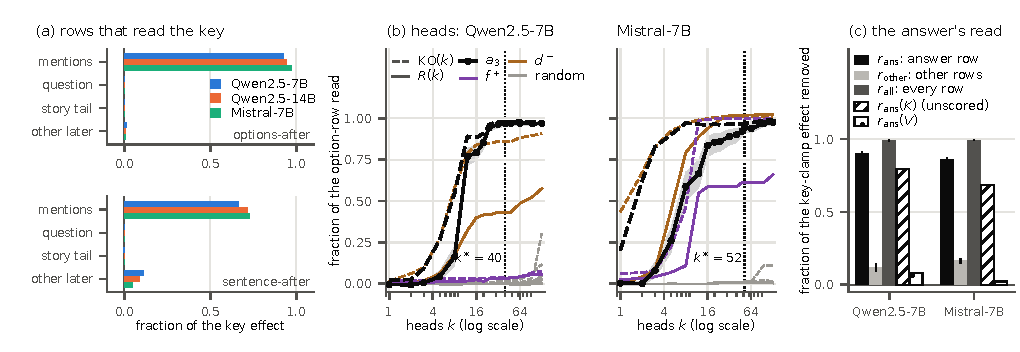
\includegraphics[width=\textwidth]{figures/fig_readers.pdf}
  \caption{\textbf{The later mentions read the writing token's key through a small set of heads, and the answer reads the later mentions} (discovery sample). (a)~Row-restricted splice ($n = 60$; D3): the fraction of the full key effect recovered when only one group of later tokens sees the source key (top \fmtOpt{}, bottom \fmtPost{}). (b)~\fmtOpt{}, 60 held-out stories: $R(k)$ (solid) and $\mathrm{KO}(k)$ (dashed) for heads ranked by $a_3$ (band: 95\% CI), by single-head effect $f^+$ and leave-one-out effect $d^-$, and three random sets (grey); dotted: $k^*$ (H1, H2). (c)~Key-clamp effect removed when only the answer row, all other later rows or all rows get the option rows' base keys and values (H5; hatched, open: keys or values only, not scored). Values in \cref{tab:localisation,tab:heads}.}
  \label{fig:readers}
\end{figure}

\paragraph{Design.} Qwen2.5-7B (\HnHeadsQwenSeven{} heads) and Mistral-7B (\HnHeadsMistralSeven{} heads), BF16 with eager attention; \fmtOpt{} confirmatory, \fmtPost{} reported. Heads are ranked on 60 ranking stories by $a_3$, the attention change of the option rows of S and B towards $p$ under the key clamp ($a_3 = \tfrac12[(A^{K_{\mathrm{S}}} - A^{\mathrm{B}})_{\text{row S} \to p} + (A^{\mathrm{B}} - A^{K_{\mathrm{S}}})_{\text{row B} \to p}]$), and every curve is evaluated on 60 other stories. $R(k)$ is the fraction of the option rows' key effect $d_G$ recovered when only the top $k$ heads see the source key in the option rows (HeadSplice; \cref{app:impl}), and $\mathrm{KO}(k)$ the fraction lost when only they are blinded; $k^* = \lceil 0.05 \times \text{heads} \rceil$ = \HkstarQwenSeven{} and \HkstarMistralSeven{}, and $k_{80}$ is the smallest $k$ on the grid with $R(k) \geq 0.8$. The other rankings are the single-head effect $f^+$ (each head alone sees the source key) and the leave-one-out effect $d^-$ (each head alone is blinded); the controls are three random sets (the first $k^*$ heads of fixed random permutations) and the $k^*$ heads most active at the option rows outside the top $2k^*$ by $a_3$. The duplicate-token score $D$ and the induction score $I$ come from 100 random repeated-token sequences, and the in-task score $T_{\mathrm{dup}}$ is the attention from each option row to the earlier occurrences of the same word other than $p$. The causal set $C$ is the top $\min(k_{80}, k^*)$ heads by $a_3$. \Cref{tab:heads} gives H1--H5, \cref{fig:heads-app} the curves and \cref{tab:ablation} every ablation condition.

\begin{table}[!ht]
\centering
\small
\caption{\textbf{Reader heads and the second hop} (preregistration H, part (a); \fmtOpt{}, 60 held-out stories, BF16). $R(k^*)$, $\mathrm{KO}(k^*)$: fraction of the option rows' key effect recovered when only the top $k^*$ heads by $a_3$ see the source key, or lost when only they are blinded. $\rho_K$: $\mathrm{ID}_K$ under mean-ablation of these heads at the option rows, relative to no ablation. $C$: the top heads by $a_3$ that carry 80\% of the read. $r_{\mathrm{ans}}$: fraction of the key-clamp effect removed when only the answer row gets the option rows' base keys and values; $r_{\mathrm{other}}$, $r_{\mathrm{all}}$: the same for every other later row and for all rows. 95\% bootstrap CIs over stories. The last row is H5's secondary contrast, reported, not scored.}
\label{tab:heads}
\begin{tabular}{@{}llcc@{}}
\toprule
 & Quantity (\fmtOpt{}) & Qwen2.5-7B & Mistral-7B \\
\midrule
 & heads $k^*$ (of all heads) & 40 (784) & 52 (1024) \\
\midrule
H1 & $R(k^*)$, top-$k^*$ by $a_3$ see $K_S$ & \begin{tabular}[t]{@{}c@{}}0.967\\[-1pt]{\scriptsize[0.952, 0.982]}\end{tabular} & \begin{tabular}[t]{@{}c@{}}0.942\\[-1pt]{\scriptsize[0.919, 0.961]}\end{tabular} \\
 & $k_{80}$ by $a_3$ / by $f^+$ / by $d^-$ & 20 / none / none & 16 / none / 12 \\
\midrule
H2 & $\mathrm{KO}(k^*)$, top-$k^*$ blinded & \begin{tabular}[t]{@{}c@{}}0.977\\[-1pt]{\scriptsize[0.966, 0.987]}\end{tabular} & \begin{tabular}[t]{@{}c@{}}0.971\\[-1pt]{\scriptsize[0.954, 0.984]}\end{tabular} \\
 & random sets: $R$ / $\mathrm{KO}$ (mean of 3) & 0.004 / 0.011 & 0.007 / 0.010 \\
\midrule
H3 & $\rho_K$ under mean-ablation of the top-$k^*$ & \begin{tabular}[t]{@{}c@{}}0.238\\[-1pt]{\scriptsize[0.205, 0.270]}\end{tabular} & \begin{tabular}[t]{@{}c@{}}0.059\\[-1pt]{\scriptsize[0.040, 0.079]}\end{tabular} \\
 & $\rho_K$, control sets (min--max) & 0.953--1.018 & 1.002--1.009 \\
 & rise of $\mathrm{ID}_V$ (nats) & \begin{tabular}[t]{@{}c@{}}$+$6.907\\[-1pt]{\scriptsize[6.264, 7.561]}\end{tabular} & \begin{tabular}[t]{@{}c@{}}$+$10.861\\[-1pt]{\scriptsize[9.995, 11.677]}\end{tabular} \\
 & answer kept (base argmax) & 0.87 & 1.00 \\
\midrule
H4 & $|C|$ (top heads by $a_3$ carrying 80\,\%) & 20 & 16 \\
 & median duplicate score $D$ over $C$ & \begin{tabular}[t]{@{}c@{}}0.370\\[-1pt]{\scriptsize[0.361, 0.378]}\end{tabular} & \begin{tabular}[t]{@{}c@{}}0.232\\[-1pt]{\scriptsize[0.227, 0.238]}\end{tabular} \\
 & median induction score $I$ over $C$ & 0.011 & 0.022 \\
 & median in-task $T_{\mathrm{dup}}$ over $C$ & 0.459 & 0.433 \\
 & top-10 by $a_3$ $\cap$ top-10 by $D$ & 6 & 5 \\
\midrule
H5 & $r_{\mathrm{ans}}$: only the answer row restored & \begin{tabular}[t]{@{}c@{}}0.899\\[-1pt]{\scriptsize[0.886, 0.913]}\end{tabular} & \begin{tabular}[t]{@{}c@{}}0.859\\[-1pt]{\scriptsize[0.845, 0.872]}\end{tabular} \\
 & $r_{\mathrm{other}}$ / $r_{\mathrm{all}}$ & 0.118 / 0.992 & 0.165 / 0.992 \\
 & $r_{\mathrm{ans}}(K)$ / $r_{\mathrm{ans}}(V)$ (secondary, not scored) & 0.797 / 0.080 & 0.683 / 0.023 \\
\bottomrule
\end{tabular}

\end{table}

\begin{figure}[!ht]
\centering
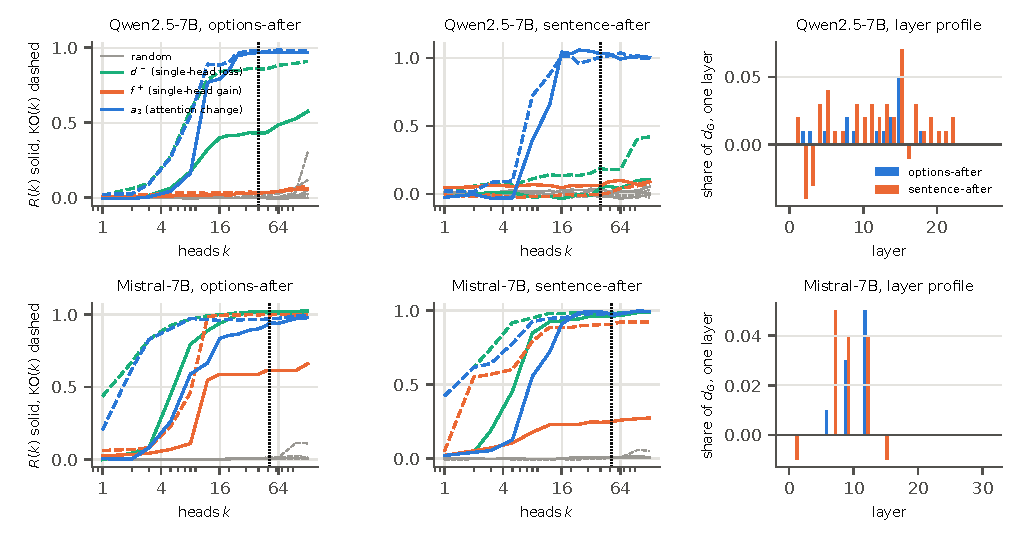
\includegraphics[width=\textwidth]{figures/fig_heads_app.pdf}
\caption{\textbf{Head curves and layer profiles} (preregistration H, part (a); exploratory except $R(k^*)$ and $\mathrm{KO}(k^*)$ of the $a_3$ ranking under \fmtOpt{}). Left and middle: $R(k)$ (solid) and $\mathrm{KO}(k)$ (dashed) against the number of heads $k$ for the rankings by $a_3$, single-head effect $f^+$ and leave-one-out effect $d^-$, and for three random sets (grey), under \fmtOpt{} and \fmtPost{}; dotted: $k^*$. Right: the share of the option rows' key effect recovered when all heads of one layer see the source key. 60 held-out stories per model and format.}
\label{fig:heads-app}
\end{figure}

\paragraph{Sufficiency and necessity (H1, H2).} The top 5\% of heads recover almost all of the option rows' read and blinding them removes almost all of it, while random sets of equal size do neither; no single random draw exceeds $R$ = \HtwoRrandMaxQwenSeven{} / \HtwoRrandMaxMistralSeven{} or $\mathrm{KO}$ = \HtwoKOrandMaxQwenSeven{} / \HtwoKOrandMaxMistralSeven{} (exploratory, recomputed). The ranking is stable: the split-half Spearman correlation of $a_3$ between ranking and evaluation stories is \HsplitOptQwenSeven{} / \HsplitOptMistralSeven{} under \fmtOpt{} and \HsplitPostQwenSeven{} / \HsplitPostMistralSeven{} under \fmtPost{}.

\paragraph{The read is a joint property of many heads (exploratory).} Ranking by single-head effect does not find the set, and ranking by leave-one-out effect finds it at one of the two models: at Qwen2.5-7B, $f^+$ reaches only $R(128)$ = \HcurveRFplusHundredandtwentyeightOptQwenSeven{} and $d^-$ \HcurveRDminusHundredandtwentyeightOptQwenSeven{}; at Mistral-7B $f^+$ reaches \HcurveRFplusHundredandtwentyeightOptMistralSeven{}, while $d^-$ reaches $k_{80}$ = \HoneKeightyDminusMistralSeven{}, fewer heads than $a_3$ needs (\HoneKeightyMistralSeven{}). The $a_3$ curve rises steeply (Qwen2.5-7B: $R(8)$ = \HcurveRAthreeEightOptQwenSeven{}, $R(12)$ = \HcurveRAthreeTwelveOptQwenSeven{}), and at Mistral-7B blinding the top three heads removes \HcurveKOAthreeThreeOptMistralSeven{} of the read while the same three alone recover \HcurveRAthreeThreeOptMistralSeven{}. Letting all heads of a single layer read the source key recovers at most \HlayerMaxOptQwenSeven{} (layer \HlayerArgOptQwenSeven{}) and \HlayerMaxOptMistralSeven{} (layer \HlayerArgOptMistralSeven{}) of $d_G$, and the single-layer shares sum to only \HlayerSumOptQwenSeven{} and \HlayerSumOptMistralSeven{} (exploratory, recomputed); the heads of $C$ span \HlayerSpanQwenSeven{} and \HlayerSpanMistralSeven{} layers (exploratory, recomputed). No single head or layer is necessary or sufficient; the top \HfourKCQwenSeven{} and \HfourKCMistralSeven{} heads by $a_3$, over many layers, are, jointly.

\begin{table}[!ht]
\centering
\caption{\textbf{Every ablation condition} (preregistration H, part (a); 60 held-out stories). $\rho_K$: $\mathrm{ID}_K$ under ablation at the six option rows, relative to none; $\Delta\mathrm{ID}_V$: rise of the value identity (nats); kept: fraction of stories whose candidate-restricted clean answer is still B. ``mean'': mean-ablation with the head's position-matched mean over the ranking stories; ``zero'': zero-ablation. H3 uses the top-$k^*$ mean row, the three random sets and the most-active set under \fmtOpt{}; every other cell is exploratory.}
\label{tab:ablation}
\resizebox{\textwidth}{!}{\begin{tabular}{@{}lcccccccccccc@{}}
\toprule
Condition & \multicolumn{3}{c}{Qwen2.5-7B, \fmtOpt{}} & \multicolumn{3}{c}{Qwen2.5-7B, \fmtPost{}} & \multicolumn{3}{c}{Mistral-7B, \fmtOpt{}} & \multicolumn{3}{c}{Mistral-7B, \fmtPost{}} \\
\cmidrule(lr){2-4}\cmidrule(lr){5-7}\cmidrule(lr){8-10}\cmidrule(lr){11-13}
 & $\rho_K$ & $\Delta\mathrm{ID}_V$ & kept & $\rho_K$ & $\Delta\mathrm{ID}_V$ & kept & $\rho_K$ & $\Delta\mathrm{ID}_V$ & kept & $\rho_K$ & $\Delta\mathrm{ID}_V$ & kept \\
\midrule
none & 1.000 & $+$0.000 & 0.97 & 1.000 & $+$0.000 & 1.00 & 1.000 & $+$0.000 & 1.00 & 1.000 & $+$0.000 & 1.00 \\
top-$k^*$ (mean) & 0.238 & $+$6.907 & 0.87 & $-$0.080 & $+$2.295 & 1.00 & 0.059 & $+$10.861 & 1.00 & 0.012 & $+$2.640 & 1.00 \\
top-10 (mean) & 0.859 & $+$1.978 & 0.98 & 0.616 & $+$1.436 & 1.00 & 0.139 & $+$12.326 & 1.00 & 0.233 & $+$2.302 & 0.98 \\
top-20 (mean) & 0.654 & $+$4.285 & 0.95 & 0.126 & $+$2.282 & 1.00 & 0.104 & $+$12.728 & 1.00 & 0.056 & $+$2.648 & 1.00 \\
top-$k^*$ (zero) & 0.081 & $+$11.315 & 1.00 & $-$0.060 & $+$2.756 & 1.00 & 0.057 & $+$9.030 & 0.95 & 0.006 & $+$2.609 & 1.00 \\
random set 1 & 1.002 & $+$0.091 & 0.97 & 0.969 & $+$0.081 & 1.00 & 1.002 & $-$0.096 & 1.00 & 1.003 & $+$0.048 & 1.00 \\
random set 2 & 0.978 & $+$0.851 & 1.00 & 0.655 & $+$0.820 & 1.00 & 1.009 & $-$0.292 & 1.00 & 1.289 & $-$1.563 & 1.00 \\
random set 3 & 0.953 & $+$0.241 & 0.98 & 0.975 & $+$0.114 & 1.00 & 1.006 & $-$0.326 & 1.00 & 1.100 & $-$0.336 & 1.00 \\
most active at $G$ & 1.018 & $-$0.177 & 0.97 & 0.934 & $+$0.012 & 1.00 & 1.009 & $+$0.049 & 1.00 & 0.949 & $+$0.521 & 1.00 \\
next $k^*$ by $a_3$ & 1.019 & $-$0.062 & 1.00 & 1.140 & $-$0.028 & 1.00 & 0.996 & $+$0.173 & 1.00 & 0.823 & $+$0.682 & 1.00 \\
\bottomrule
\end{tabular}
}
\end{table}

\paragraph{Ablation (H3).} Mean-ablating the top-$k^*$ heads at the option rows removes most of the key identity, raises the value identity and keeps the answer; the random and most-active sets of equal size leave $\rho_K$ near 1 (\cref{tab:ablation}). Zero-ablation (exploratory) goes the same way ($\rho_K$ = \HablTopkzeroRhoOptQwenSeven{} and \HablTopkzeroRhoOptMistralSeven{}). Without ablation the answer is B in \HablNoneBaseOptQwenSeven{} of Qwen2.5-7B stories, against \HthreeBaseQwenSeven{} under ablation. The rise of the value identity is partial at Qwen2.5-7B ($\mathrm{ID}_V$ under ablation \HablIDVafterQwenSeven{} nats against \idVNoneQwenSeven{} under \fmtNone{} in stage 1), and at Mistral-7B it reaches about the \fmtNone{} level (\HablIDVafterMistralSeven{} against \idVNoneMistralSeven{}); both comparisons are across stages and stories (arithmetic on printed values). The stage-5 edge knockout keeps the answer only at Qwen2.5-14B (G7b); the two interventions differ (mean-ablation at six rows leaves $\rho_K$ = \HthreeRhoQwenSeven{} at Qwen2.5-7B, the knockout leaves $r_K \approx 0$), and we do not reconcile them.

\paragraph{Duplicate-token heads (H4) and the size of $C$.} Over $C$ the median previous-token score is \HcPrevOptQwenSeven{} / \HcPrevOptMistralSeven{} (largest \HfourPrevMaxQwenSeven{} / \HfourPrevMaxMistralSeven{}, exploratory, recomputed), and the in-task score of control words that are not candidates is \HcTctrlOptQwenSeven{} / \HcTctrlOptMistralSeven{}, against $T_{\mathrm{dup}}$ = \HfourTQwenSeven{} / \HfourTMistralSeven{}. $T_{\mathrm{dup}}$ is measured in the task the heads were selected on, so we treat it as supporting rather than independent evidence; $D$ and $I$, on random sequences, are the test. H4 depends on the size of the head set (exploratory, recomputed): only \HfourNDgeQwenSeven{} of the \HfourKCQwenSeven{} heads of $C$ at Qwen2.5-7B and \HfourNDgeMistralSeven{} of the \HfourKCMistralSeven{} at Mistral-7B have $D \geq 0.2$, against \HfourNDgeWholeQwenSeven{} and \HfourNDgeWholeMistralSeven{} in the whole model, whose median $D$ is \HfourDwholeQwenSeven{} / \HfourDwholeMistralSeven{}. Over the full top-$k^*$ set (exploratory) the median $D$ is \HfourDkstarQwenSeven{} / \HfourDkstarMistralSeven{}; at Mistral-7B it is \HfourDtopTwentyMistralSeven{} over the top 20 and \HfourDtopTwelveMistralSeven{} over the top 12. At Qwen2.5-7B (exploratory), $R(16)$ = \HoneRsixteenQwenSeven{}, just under 0.8, so $C$ has 20 heads; over the top 16 the median $D$ would also be \HfourDtopSixteenQwenSeven{}. Over all heads, $a_3$ correlates weakly with $D$ (Spearman \HfourRhoDQwenSeven{} / \HfourRhoDMistralSeven{}) and with $T_{\mathrm{dup}}$ (\HfourRhoTQwenSeven{} / \HfourRhoTMistralSeven{}). We therefore say that the core of the readers, the top heads by $a_3$ that carry 80\% of the read, is canonical duplicate-token heads, not that every reader is one.

\paragraph{The second hop in detail (H5).} The routes add up: $r_{\mathrm{ans}} + r_{\mathrm{other}}$ = \HhopSumOptQwenSeven{} / \HhopSumOptMistralSeven{} against $r_{\mathrm{all}}$ = \HfiveAllQwenSeven{} / \HfiveAllMistralSeven{}. Restricted to single option rows, the source word's row gives $r_{\mathrm{ans}}$ = \HhoprowRowsAnsKVOptQwenSeven{} / \HhoprowRowsAnsKVOptMistralSeven{}, the base word's row \HhoprowRowbAnsKVOptQwenSeven{} / \HhoprowRowbAnsKVOptMistralSeven{} and the separators \HhoprowSepAnsKVOptQwenSeven{} / \HhoprowSepAnsKVOptMistralSeven{} (exploratory). As H5's secondary contrast, reported and not scored, the answer reads the option rows mainly through their keys ($r_{\mathrm{ans}}(K) - r_{\mathrm{ans}}(V)$ = \HfiveKminusVQwenSeven{} / \HfiveKminusVMistralSeven{}, CIs excluding zero), and the strong version $r_{\mathrm{ans}}(KV) \geq 0.7$ holds in both models.

\paragraph{\fmtPost{} (reported, not scored).} Gate a2 failed at Qwen2.5-7B under \fmtPost{} (\cref{app:prereg}), so H6 and H5's \fmtPost{} line are not evaluable; the values below are exploratory. The option-row ceiling covers less of the full effect than under \fmtOpt{} ($d_G/d_{\mathrm{full}}$ = \HathreeRatioPostQwenSeven{} / \HathreeRatioPostMistralSeven{}, exploratory, recomputed). At Qwen2.5-7B, $R(k)$ and $\mathrm{KO}(k)$ exceed 1 (\cref{fig:heads-app}), and mean-ablation of the top $k^*$ drives $\rho_K$ to $\HablTopkRhoPostQwenSeven$; one random set changes $\rho_K$ substantially in each model (\cref{tab:ablation}). The answer row's read gives $r_{\mathrm{ans}}$ = \HfivesAnsQwenSeven{} / \HfivesAnsMistralSeven{}, mainly through keys ($r_{\mathrm{ans}}(K)$ = \HhopAnsKPostQwenSeven{} / \HhopAnsKPostMistralSeven{}, $r_{\mathrm{ans}}(V)$ = $\HhopAnsVPostQwenSeven$ / \HhopAnsVPostMistralSeven{}). The top-20 heads by $a_3$ of the two formats share \HsixOverlapQwenSeven{} and \HsixOverlapMistralSeven{} heads (H6's threshold is 10; met at Mistral-7B, not evaluable at Qwen2.5-7B), the top 10 share \HcrossToptenQwenSeven{} and \HcrossToptenMistralSeven{}, and the full $a_3$ grids correlate at Spearman \HcrossRhoQwenSeven{} / \HcrossRhoMistralSeven{} (exploratory, recomputed). In this free-form format the candidates carry little of the clean answer's probability, so H3's candidate-mass criterion fails in every condition, as expected.

\paragraph{Ablation against knockout (not reconciled).} Mean-ablating the reader heads at the six option rows (H3) keeps the base answer, while cutting the candidate words' attention to the writing token (G5) keeps it only at Qwen2.5-14B (G7b): the two interventions differ, and the discovery sample does not reconcile them. The passage tests of the final round that would have bridged them were not evaluable (\cref{app:natural}).

\subsection{What the reader heads write: the flag}\label{app:flag}

\begin{figure}[!ht]
  \centering
  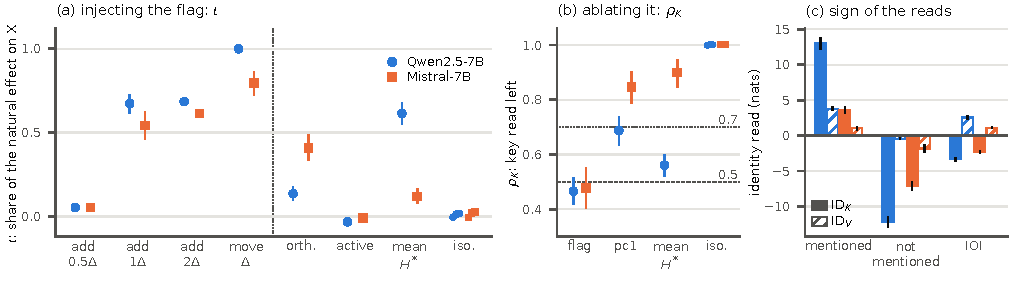
\includegraphics[width=\textwidth]{figures/fig_flag.pdf}
  \caption{\textbf{What the reader heads write.} Qwen2.5-7B and Mistral-7B; flags fit on 60 discovery-sample stories, tested on 100 others (60 in (b)); 95\,\% story-bootstrap intervals, the fit fixed. (a)~$\iota$: effect on an absent option X relative to the natural key clamp's, for the flag ($\Delta$) added 0.5, 1 or 2 times at X's row (exploratory) or moved there from B's row, and for controls: orth., the story's own write without its flag component; active, the flag of the most active heads; mean $H^*$, the reader heads' mean output; iso., isotropic directions. (b)~$\rho_K$: key read left when one direction per layer is removed at the option rows (pc1: the heads' top principal direction); dashed, dotted: the bounds for the flag and the controls. (c)~$\mathrm{ID}_K$, $\mathrm{ID}_V$ when asked which option is or is not mentioned, and in IOI.}
  \label{fig:flag}
\end{figure}

\paragraph{Definitions.} Let $H^*$ be the reader heads of the discovery sample (the top 5\,\% by $a_3$ under \fmtOpt{}, frozen: 40 heads at Qwen2.5-7B, 52 at Mistral-7B). Under the natural key clamp $K_{\mathrm{S}}$, the heads' summed write at layer $l$ into the rows of S and B changes; the \emph{flag} $\Delta_l$ is the mean over the 60 ranking stories of half the sum of the change at S's row and minus the change at B's row, projected through each head's output matrix, one vector per layer that holds an $H^*$ head. Leave-one-word-out flags $\Delta^{-w}$ are fit on the stories in which $w$ is neither B nor S. An \emph{injection} adds a vector to the attention output at chosen rows, in the clean base run, with no key clamp; ``move'' adds the flag at an option's row and subtracts it at B's row. With $\ell_w$ the six-way log-probability of candidate $w$ and $N_X$ the natural key clamp's effect on X, $\iota$ = the injection's mean effect on $\ell_X$ divided by $N_X$; $\pi_X$ = the share of stories whose answer becomes X; $\mathrm{ID}_{\mathrm{inj}}$ = the identity contrast of moving the flag to S against X; $\rho_K(u)$ = $\mathrm{ID}_K$ with the direction $u$ removed at the six option rows, relative to none; $r_{\mathrm{ans}}^{\mathrm{inj}}(C)$ = the share of the injection's effect removed when only the answer row reads the option rows' clean channel $C$. Scale (\cref{app:scale}): $\omega$, how far the flag written in a sentence matches the list's along the list flag; $c_{\mathrm{fl}}$, the cosine of the sentence and list flags; $\rho$ and $\rho_{\mathrm{nat}}$, the injected and natural sentence-to-list ratios. Binding: $\Psi_{\mathrm{bind}}$, the double difference of initial-state flags under two binding questions. The runs are BF16 with sdpa attention, except the passes that fix the head sets (eager), and every ratio is taken within one run; the intervals are over stories, conditional on the fitted flag and the frozen heads. \Cref{tab:flag} gives every line. The intervals of this subsection resample stories with the flag's fit held fixed: they exclude the uncertainty of the fit itself, which matters because several criteria were decided near their thresholds: J-D2's differences (0.385 and 0.384 against 0.4), Qwen2.5-7B's $\rho_K$ of the top principal direction (\JdThreeRhoPconeQwenSeven{} against 0.7) and Mistral-7B's $\rho_K$ of the flag (\JdThreeRhoFlagMistralSeven{} against 0.5). These decisions lie within an uncertainty the intervals do not show, and J-D1's intervals are narrower than a refit inside each resample would give; that refit was not run. % verbatim: "0.385 / 0.384 against 0.4", outcome J part D % verbatim: 40 and 52 heads, entry J part D

\begin{table}[!ht]
\centering
\caption{\textbf{The flag: every line of the mechanism tests.} Top: Qwen2.5-7B and Mistral-7B, flags fit on 60 discovery-sample stories and tested on 100 new ones (the ablations of J-D3 on the first 60 of them); bottom: the scale lines at Qwen2.5-1.5B, 3B and 7B (\cref{app:scale}). 95\,\% story-bootstrap intervals. $Q_{\mathrm{IN}}$, $Q_{\mathrm{OUT}}$: \fmtOpt{} asked which option is (is not) mentioned; IOI in-sentence: the four names listed right after the indirect object's mention (\cref{app:sign}). n.e.: not evaluable (gate in brackets). $^\dagger$Recomputed: at 3B the line is not evaluable (too few competent cores), and the post hoc rows are not printed by the scorer.}
\label{tab:flag}
\scalebox{0.8}{\begin{minipage}{1.2\textwidth}\centering\footnotesize
\setlength{\tabcolsep}{4pt}
\begin{tabular}{@{}lllll@{}}
\toprule
Line & Statistic & Qwen2.5-7B & Mistral-7B & Verdict \\
\midrule
J-D1 & $\mathrm{ID}^{\mathrm{LOO}}_{\mathrm{inj}}/\mathrm{ID}_K$ & 0.997 [0.980, 1.014] & 0.803 [0.746, 0.856] & \textbf{met} \\
 & $\pi_X$ & 0.96 & 0.67 &  \\
J-D2 & $\iota$(move $\Delta$) & 0.999 [0.992, 1.006] & 0.794 [0.719, 0.864] & \textbf{not met} \\
 & $\iota$(own write $\perp$ flag) & 0.135 [0.096, 0.179] & 0.409 [0.332, 0.488] &  \\
 & $\iota$(mean $H^*$ output) & 0.614 [0.549, 0.679] & 0.120 [0.078, 0.166] &  \\
 & $\iota$(active-set flag) & $-$0.032 [$-$0.037, $-$0.027] & $-$0.010 [$-$0.015, $-$0.006] &  \\
J-D3 & $\rho_K$(flag) & 0.466 [0.416, 0.516] & 0.478 [0.403, 0.553] & \textbf{not met} \\
 & $\rho_K$(pc1) & 0.687 [0.633, 0.738] & 0.846 [0.786, 0.902] &  \\
 & $\rho_K$(mean $H^*$ output) & 0.561 [0.520, 0.600] & 0.899 [0.846, 0.946] &  \\
J-D4 & $r^{\mathrm{inj}}_{\mathrm{ans}}(KV)$ & 0.869 [0.855, 0.884] & 0.762 [0.737, 0.786] & \textbf{met} \\
 & $r^{\mathrm{inj}}_{\mathrm{ans}}(K)$ & 0.689 [0.642, 0.735] & 0.601 [0.540, 0.659] &  \\
 & $r^{\mathrm{inj}}_{\mathrm{ans}}(V)$ & 0.047 [0.030, 0.067] & 0.068 [0.035, 0.104] &  \\
 & $r^{\mathrm{inj}}_{\mathrm{ans}}(K) - r^{\mathrm{inj}}_{\mathrm{ans}}(V)$ & 0.642 [0.589, 0.692] & 0.533 [0.478, 0.588] &  \\
J-D-ADDR & weighted $\cos(\Delta^K, \Delta^{KV})$ & 0.993 & 0.962 & \textbf{met} \\
 & $\mathrm{ID}_{\mathrm{inj}}(KV)/\mathrm{ID}_{\mathrm{inj}}(K)$ & 1.005 [1.003, 1.008] & 0.981 [0.949, 1.013] &  \\
J-D-KN & Pearson (per story) & 0.894 [0.868, 0.917] & 0.147 [0.041, 0.252] & \textbf{not met} \\
 & B-loss ratio $\beta$ & 5.167 [3.878, 7.704] & 9.095 [2.862, 58.110] &  \\
 & mean$(\Delta\ell_S - \Delta\ell_X)$ (nats) & $-$0.073 [$-$0.763, 0.612] & 0.290 [$-$0.457, 1.024] &  \\
J-D5 & $\Psi_{\mathrm{bind}}$ pooled (nats) & $-$0.578 [$-$0.863, $-$0.308] & 0.269 [0.096, 0.456] & \textbf{not met} \\
 & object-first & 0.376 [0.156, 0.619] & 0.459 [0.120, 0.848] &  \\
 & distractor-first & $-$1.299 [$-$1.678, $-$0.955] & 0.126 [$-$0.034, 0.283] &  \\
 & stratum difference & 1.675 [1.272, 2.115] & 0.333 [$-$0.049, 0.751] &  \\
J-D7 & $\mathrm{ID}_K(Q_{\mathrm{OUT}})$ (nats) & $-$12.138 [$-$12.905, $-$11.413] & $-$7.083 [$-$7.726, $-$6.463] & \textbf{met} \\
 & $\mathrm{ID}_K(Q_{\mathrm{IN}})$ (nats) & 13.005 [12.206, 13.777] & 3.575 [3.085, 4.059] &  \\
 & paired difference (nats) & 25.143 [24.121, 26.159] & 10.658 [9.897, 11.413] &  \\
J-D-SIGN-Q & $\mathrm{ID}_V(Q_{\mathrm{OUT}})$ (nats) & $-$0.431 [$-$0.616, $-$0.254] & $-$1.806 [$-$2.442, $-$1.192] & \textbf{met} \\
J-D-SIGN-IOI & $\mathrm{ID}_K$, IOI in-sentence (nats) & $-$3.350 [$-$3.655, $-$3.042] & $-$2.352 [$-$2.542, $-$2.162] & \textbf{met} \\
 & $\mathrm{ID}_V$, IOI in-sentence (nats) & 2.550 [2.244, 2.889] & 1.096 [0.945, 1.247] &  \\
J-D8-Q & $R(H^*)$, $Q_{\mathrm{IN}}$ & 1.027 [1.016, 1.038] & 1.058 [1.032, 1.087] & \textbf{met} \\
 & $\mathrm{KO}(H^*)$, $Q_{\mathrm{IN}}$ & 0.974 [0.968, 0.980] & 0.931 [0.892, 0.964] &  \\
 & $R(H^*)$, $Q_{\mathrm{OUT}}$ & 0.986 [0.971, 1.002] & 1.050 [1.011, 1.093] &  \\
 & $\mathrm{KO}(H^*)$, $Q_{\mathrm{OUT}}$ & 1.021 [1.001, 1.041] & 0.958 [0.918, 0.995] &  \\
J-D8-IOI & $R(H^*)$, IOI in-sentence & 0.922 [0.882, 0.960] & n.e.\ (J-D-G4 INLINE) & \textbf{not evaluable} \\
 & $\mathrm{KO}(H^*)$, IOI in-sentence & 0.998 [0.980, 1.016] & n.e.\ (J-D-G4 INLINE) &  \\
J-D-ROUTE-IOI & $r_{\mathrm{ans}}(KV)$ & 0.897 [0.821, 0.976] & 0.839 [0.769, 0.910] & \textbf{met} \\
 & $r_{\mathrm{ans}}(K)$ & 0.431 [0.318, 0.536] & 0.488 [0.406, 0.567] &  \\
 & $r_{\mathrm{ans}}(V)$ & 0.211 [0.163, 0.267] & 0.263 [0.231, 0.298] &  \\
 & $r_{\mathrm{ans}}(K) - r_{\mathrm{ans}}(V)$ & 0.220 [0.081, 0.343] & 0.225 [0.131, 0.314] &  \\
 & $r_{\mathrm{other}}$ & 0.103 [0.064, 0.146] & 0.190 [0.157, 0.223] &  \\
J-D-HOP2 & carry, top-10 hop-2 heads, $Q_{\mathrm{OUT}}$ & 0.077 [0.062, 0.092] & 0.161 [0.117, 0.208] & \textbf{not met} \\
 & carry, top-10 hop-2 heads, IOI & $-$0.085 [$-$0.141, $-$0.036] & $-$0.029 [$-$0.093, 0.025] &  \\
\bottomrule
\end{tabular}

\medskip

\begin{tabular}{@{}llcccl@{}}
\toprule
Line & Statistic & Qwen2.5-1.5B & Qwen2.5-3B & Qwen2.5-7B & Verdict \\
\midrule
J-D6a & $\omega$ & \begin{tabular}[t]{@{}c@{}}0.967\\[-1pt]{\scriptsize[0.952, 0.982]}\end{tabular} & \begin{tabular}[t]{@{}c@{}}0.954\\[-1pt]{\scriptsize[0.937, 0.971]}\end{tabular} & \begin{tabular}[t]{@{}c@{}}0.822\\[-1pt]{\scriptsize[0.810, 0.834]}\end{tabular} & \textbf{met} \\
 & $c_{\mathrm{fl}}$ & 0.966 & 0.895 & 0.872 &  \\
J-D6 & $\rho$ & \begin{tabular}[t]{@{}c@{}}$-$0.126\\[-1pt]{\scriptsize[$-$0.179, $-$0.077]}\end{tabular} & \begin{tabular}[t]{@{}c@{}}$-$0.025$^\dagger$ (n.e.)\\[-1pt]{\scriptsize [$-$0.104, 0.050]}\end{tabular} & \begin{tabular}[t]{@{}c@{}}0.257\\[-1pt]{\scriptsize[0.222, 0.292]}\end{tabular} & \textbf{not met} \\
 & $\rho_{\mathrm{nat}}$ & \begin{tabular}[t]{@{}c@{}}0.090\\[-1pt]{\scriptsize[0.042, 0.137]}\end{tabular} & \begin{tabular}[t]{@{}c@{}}0.266$^\dagger$ (n.e.)\\[-1pt]{\scriptsize [0.196, 0.341]}\end{tabular} & \begin{tabular}[t]{@{}c@{}}0.468\\[-1pt]{\scriptsize[0.431, 0.505]}\end{tabular} &  \\
 & $\rho - \rho_{\mathrm{nat}}$ & \begin{tabular}[t]{@{}c@{}}$-$0.216\\[-1pt]{\scriptsize[$-$0.273, $-$0.163]}\end{tabular} & \begin{tabular}[t]{@{}c@{}}$-$0.290$^\dagger$ (n.e.)\\[-1pt]{\scriptsize [$-$0.376, $-$0.213]}\end{tabular} & \begin{tabular}[t]{@{}c@{}}$-$0.211\\[-1pt]{\scriptsize[$-$0.245, $-$0.178]}\end{tabular} &  \\
J-D6-ROUTE & $r^{\mathrm{inj}}_{\mathrm{ans}}(V)$ & \begin{tabular}[t]{@{}c@{}}$-$0.140\\[-1pt]{\scriptsize[$-$0.276, $-$0.054]}\end{tabular} & -- & -- & \textbf{not met} \\
 & $r^{\mathrm{inj}}_{\mathrm{ans}}(K)$ & \begin{tabular}[t]{@{}c@{}}1.114\\[-1pt]{\scriptsize[1.006, 1.285]}\end{tabular} & -- & -- &  \\
 & $r^{\mathrm{inj}}_{\mathrm{ans}}(V) - r^{\mathrm{inj}}_{\mathrm{ans}}(K)$ & \begin{tabular}[t]{@{}c@{}}$-$1.254\\[-1pt]{\scriptsize[$-$1.543, $-$1.075]}\end{tabular} & -- & -- &  \\
J-D6, post hoc & natural ratio, $X$-specific contrast$^\dagger$ & \begin{tabular}[t]{@{}c@{}}$-$0.113\\[-1pt]{\scriptsize[$-$0.213, $-$0.030]}\end{tabular} & -- & \begin{tabular}[t]{@{}c@{}}0.271\\[-1pt]{\scriptsize[0.234, 0.308]}\end{tabular} & -- \\
 & $\rho$ minus it$^\dagger$ & \begin{tabular}[t]{@{}c@{}}$-$0.013\\[-1pt]{\scriptsize[$-$0.099, 0.083]}\end{tabular} & -- & \begin{tabular}[t]{@{}c@{}}$-$0.014\\[-1pt]{\scriptsize[$-$0.049, 0.022]}\end{tabular} &  \\
 & natural ratio on $\mathrm{ID}_K$$^\dagger$ & \begin{tabular}[t]{@{}c@{}}$-$0.115\\[-1pt]{\scriptsize[$-$0.182, $-$0.062]}\end{tabular} & -- & \begin{tabular}[t]{@{}c@{}}0.290\\[-1pt]{\scriptsize[0.270, 0.311]}\end{tabular} &  \\
 & $\rho$ minus it$^\dagger$ & \begin{tabular}[t]{@{}c@{}}$-$0.011\\[-1pt]{\scriptsize[$-$0.079, 0.061]}\end{tabular} & -- & \begin{tabular}[t]{@{}c@{}}$-$0.033\\[-1pt]{\scriptsize[$-$0.066, $-$0.002]}\end{tabular} &  \\
D6b & $\Delta^{\mathrm{sentence}}/\Delta^{\mathrm{list}}$ at the list row & \begin{tabular}[t]{@{}c@{}}0.926\\[-1pt]{\scriptsize[0.908, 0.942]}\end{tabular} & \begin{tabular}[t]{@{}c@{}}0.926\\[-1pt]{\scriptsize[0.892, 0.961]}\end{tabular} & \begin{tabular}[t]{@{}c@{}}0.943\\[-1pt]{\scriptsize[0.924, 0.961]}\end{tabular} & reported \\
\bottomrule
\end{tabular}
\end{minipage}}
\end{table}

\paragraph{Sufficiency and identity (J-D1, risky, held; J-D-ADDR, held).} Moved into the row of an option absent from the story (added there and subtracted at B's row, as the natural key clamp moves it), the flag fit without that option's word moves the answer there: $\mathrm{ID}_{\mathrm{inj}}^{\mathrm{LOO}}/\mathrm{ID}_K$ = \JdOneRatioQwenSeven{} [\JdOneRatioQwenSevenLo{}, \JdOneRatioQwenSevenHi{}] and \JdOneRatioMistralSeven{} [\JdOneRatioMistralSevenLo{}, \JdOneRatioMistralSevenHi{}], and the answer changes in $\pi_X$ = \JdOnePiXQwenSeven{} and \JdOnePiXMistralSeven{} of stories. The mean flag names no candidate: fit from the natural source run instead of the key clamp it is the same direction (norm-weighted cosine \JdAddrCosQwenSeven{} and \JdAddrCosMistralSeven{}) with the same effect (ratio \JdAddrRatioQwenSeven{} [\JdAddrRatioQwenSevenLo{}, \JdAddrRatioQwenSevenHi{}] and \JdAddrRatioMistralSeven{} [\JdAddrRatioMistralSevenLo{}, \JdAddrRatioMistralSevenHi{}]). Added alone, without the subtraction at B's row (which keeps its own flag), the flag has less effect: half a flag barely moves the answer, and one and two flags saturate below the full effect, consistent with competition among flagged rows (post hoc reading; adding half, one and two flags at X's row gives $\iota$ = \JdDoseHalfQwenSeven{}, \JdDoseOneQwenSeven{}, \JdDoseTwoQwenSeven{} and \JdDoseHalfMistralSeven{}, \JdDoseOneMistralSeven{}, \JdDoseTwoMistralSeven{}); the full flag gives $\mathrm{ID}_{\mathrm{inj}}/\mathrm{ID}_K$ = \JdFullFlagQwenSeven{} and \JdFullFlagMistralSeven{}; isotropic, head-span, layer-permuted and wrongly placed flags (at the ``Choices'' and ``Question'' rows) give $\lvert\iota\rvert \leq \JdSanityAbsMax{}$ (reported).

\paragraph{Specificity (J-D2, risky, not held).} The line required three structured controls to move the answer at most 0.3 as much as the flag. The active-set flag (the same construction over the heads most active at the option rows) does not move it ($\iota$ = \JdTwoIotaActiveQwenSeven{} and \JdTwoIotaActiveMistralSeven{}), but at Qwen2.5-7B the mean reader output at the option rows, norm-matched, moves it \JdTwoRatioMeanHQwenSeven{} as much as the flag, and at Mistral-7B the story's own write with its flag component removed, norm-matched, \JdTwoRatioOrthMistralSeven{} as much. The checks found (exploratory, recomputed) that the Qwen control overlaps the flag by construction: the clean reader output at the option rows contains the flag written at the mentioned words' rows (norm-weighted cosine 0.636), 54\,\% of the flag's energy lies along the mean-output directions and 29\,\% along the top principal direction, and ablating the mean output reproduces the flag's value-channel signature. The overlap explains much but not all of the failure (a linear energy estimate gives $\rho_K$ about 0.71 and 0.85 for the two Qwen controls), and Mistral's controls overlap the flag too (cosine 0.58) yet pass. The Mistral failure on the orthogonal own write points to a story-specific write (rank-one capture \JdRankOneMistralSeven{}, against \JdRankOneQwenSeven{} at Qwen). % verbatim: outcome J part D

\paragraph{Necessity (J-D3, risky, not held).} Removing the flag direction at the six option rows, one direction per layer, leaves $\rho_K$ = \JdThreeRhoFlagQwenSeven{} [\JdThreeRhoFlagQwenSevenLo{}, \JdThreeRhoFlagQwenSevenHi{}] and \JdThreeRhoFlagMistralSeven{} [\JdThreeRhoFlagMistralSevenLo{}, \JdThreeRhoFlagMistralSevenHi{}] of the key read: about half in both models. The line also required two control directions, the top principal direction of the heads' output and the mean reader output, to leave at least 0.7. At Mistral they do (\JdThreeRhoPconeMistralSeven{} and \JdThreeRhoMeanHMistralSeven{}) and the line holds there, with the flag's point estimate close to its 0.5 floor; at Qwen they remove 31\,\% and 44\,\% (they leave \JdThreeRhoPconeQwenSeven{} and \JdThreeRhoMeanHQwenSeven{}) because they overlap the flag, and the line fails. % verbatim: "31 % and 44 %", outcome J part D
 Isotropic directions leave \JdRhoIsoMin{}--\JdRhoIsoMax{} (reported). The pre-written replacement used in the main text: ``One direction per layer does not carry the key read ($\rho_K$ = \JdThreeRhoFlagQwenSeven{} / \JdThreeRhoFlagMistralSeven{}): other carriers exist; the flag is sufficient but not necessary.'' Whole-head ablation of the reader heads removes far more of the read (discovery sample: $\rho_K$ = \HthreeRhoQwenSeven{} and \HthreeRhoMistralSeven{}; \cref{tab:ablation}), so the heads write more than this direction. % verbatim: J-D3 text, outcome J part D

\paragraph{Read by key (J-D4, held).} Giving only the answer row the option rows' clean keys and values removes $r_{\mathrm{ans}}^{\mathrm{inj}}(KV)$ = \JdFourKVQwenSeven{} and \JdFourKVMistralSeven{} of the injected flag's effect; their clean keys alone \JdFourKQwenSeven{} and \JdFourKMistralSeven{}, their clean values alone \JdFourVQwenSeven{} and \JdFourVMistralSeven{} ($K - V$ = \JdFourKmVQwenSeven{} [\JdFourKmVQwenSevenLo{}, \JdFourKmVQwenSevenHi{}] and \JdFourKmVMistralSeven{} [\JdFourKmVMistralSevenLo{}, \JdFourKmVMistralSevenHi{}]); every other later row carries \JdFourOtherQwenSeven{} and \JdFourOtherMistralSeven{} (reported). The answer reads the injected flag by key, as it reads the natural one (discovery sample, H5).

\paragraph{What the flag is (reported).} Its largest cosine with the unembeddings of the locations is \JdLensMaxQwenSeven{} at Qwen and \JdLensMaxMistralSeven{} at Mistral (both at layer \JdLensLayerQwenSeven{}), against at most \JdLensRandMaxQwenSeven{} and \JdLensRandMaxMistralSeven{} for random token rows: it is not a readable location word. The share of the per-story flag's variance explained by the identity of B is \JdBidShareMin{}--\JdBidShareMax{} across layers, against a null of \JdBidShareNull{}: the mean flag is identity-free, while each story's write also carries its own word.

\paragraph{A key that names no candidate (J-D-KN, risky, not held).} Clamping the writing token's key to a word that is not a candidate (``garage'', ``kitchen'', \ldots) was predicted to act like removing B's flag. Per story, its effects on the six candidates correlate with those of subtracting the flag at B's row at Qwen (Pearson \JdKnPearsonQwenSeven{}) but not at Mistral (\JdKnPearsonMistralSeven{}), and the loss of support for B is far larger than the flag's ($\beta$ = \JdKnBetaQwenSeven{} and \JdKnBetaMistralSeven{} against the preregistered 0.7--1.3); the third criterion held (\JdKnDiffQwenSeven{} and \JdKnDiffMistralSeven{} nats against tolerances of \JdKnTolQwenSeven{} and \JdKnTolMistralSeven{}). The printed sizes are inflated, because at Qwen $p(\mathrm{B}) > 0.99$ in every clean story and at Mistral the denominator is nearly inert; on the six-way logit of B, $\beta$ is 1.93 [1.78, 2.10] and 5.20 [3.38, 10.49] (exploratory, recomputed): a non-candidate key removes about two (Qwen) to five (Mistral) times more support for B than subtracting the mean flag at B's row. % verbatim: outcome J part D

\paragraph{Binding (J-D5, risky, not held).} The flags of the two initial-state sentences were predicted to carry which object they bind, in both sentence orders. Pooled, $\Psi_{\mathrm{bind}}$ = \JdFivePooledQwenSeven{} [\JdFivePooledQwenSevenLo{}, \JdFivePooledQwenSevenHi{}] at Qwen (below zero) and \JdFivePooledMistralSeven{} [\JdFivePooledMistralSevenLo{}, \JdFivePooledMistralSevenHi{}] at Mistral; the two orders differ at Qwen (object first \JdFiveObjQwenSeven{}, distractor first \JdFiveDisQwenSeven{} nats; difference \JdFiveDiffQwenSeven{} [\JdFiveDiffQwenSevenLo{}, \JdFiveDiffQwenSevenHi{}]). The pre-written replacement: ``The initial-state flag does not carry binding in a way separable from order.'' The order effect is a property of the model, not of the fit (the fit set is balanced, 23 against 22 stories), and the two initial-state flags are nearly collinear (weighted cosine 0.97 in both models), so $\Psi_{\mathrm{bind}}$ is a 0.2--1.1-nat contrast on injection effects of 12--19 nats; Mistral's pass is fragile (distractor first \JdFiveDisMistralSeven{} [\JdFiveDisMistralSevenLo{}, \JdFiveDisMistralSevenHi{}]). % verbatim: outcome J part D

\paragraph{Other tasks (exploratory).} The belief flag injected into the paint and schedule tasks gives \JdXtaskPaintQwenSeven{} of the tasks' own flag at Qwen, and \JdXtaskPaintMistralSeven{} and \JdXtaskScheduleMistralSeven{} at Mistral.

\paragraph{Holm sensitivity.} Over the 27 interval components of this part's risky lines with a verdict, Holm's step-down changes no decision and no verdict. % verbatim: outcome J part D

\subsection{The sign of the read, and IOI}\label{app:sign}

\paragraph{The question sets the sign (J-D7, J-D-SIGN-Q, J-D8-Q, held).} Asked which option is \emph{not} mentioned in the story ($Q_{\mathrm{OUT}}$), the key read turns negative: $\mathrm{ID}_K$ = \JdSevenQoutQwenSeven{} [\JdSevenQoutQwenSevenLo{}, \JdSevenQoutQwenSevenHi{}] and \JdSevenQoutMistralSeven{} [\JdSevenQoutMistralSevenLo{}, \JdSevenQoutMistralSevenHi{}] nats, against \JdSevenQinQwenSeven{} and \JdSevenQinMistralSeven{} when asked which option is mentioned ($Q_{\mathrm{IN}}$; paired differences \JdSevenDiffQwenSeven{} and \JdSevenDiffMistralSeven{}). The value read turns negative too ($\mathrm{ID}_V$ = \JdSignQIDVQwenSeven{} [\JdSignQIDVQwenSevenLo{}, \JdSignQIDVQwenSevenHi{}] and \JdSignQIDVMistralSeven{} [\JdSignQIDVMistralSevenLo{}, \JdSignQIDVMistralSevenHi{}]), so the sign follows the task, not a polarity of the readers. The same frozen reader heads carry the read under both questions: when only they see the clamped key they recover $R$ = \JdEightQinRQwenSeven{} and \JdEightQinRMistralSeven{} of it under $Q_{\mathrm{IN}}$ and \JdEightQoutRQwenSeven{} and \JdEightQoutRMistralSeven{} under $Q_{\mathrm{OUT}}$, blinding them removes \JdEightQinKOQwenSeven{}--\JdEightQoutKOQwenSeven{} at Qwen and \JdEightQinKOMistralSeven{}--\JdEightQoutKOMistralSeven{} at Mistral, and random sets of the same size do neither (their $R$ and KO lie between $-0.006$ and $+0.015$). % verbatim: outcome J part D
 Behaviourally, under $Q_{\mathrm{OUT}}$ the key clamp makes the story's own location the answer in \pct{\JdQoutKSQwenSeven} and \pct{\JdQoutKSMistralSeven} of stories, and the list flag injected at X's row moves the answer \JdNineQoutRatioQwenSeven{} and \JdNineQoutRatioMistralSeven{} as much as the natural clamp (reported; under $Q_{\mathrm{IN}}$ \JdNineQinRatioQwenSeven{} and \JdNineQinRatioMistralSeven{}): the readers' write need not change with the question, and the sign is applied after the first hop (exploratory). A negative use of duplicate detection is known \citep{wang2022ioi,mcdougall2023copy}; we do not present the polarity as a discovery.

\paragraph{IOI separates the channels (J-D-SIGN-IOI, held).} In the in-sentence re-mentions of indirect-object identification (the four names listed right after the indirect object's mention), the key read is negative while the value read stays positive: $\mathrm{ID}_K$ = \JdSignIoiIDKQwenSeven{} [\JdSignIoiIDKQwenSevenLo{}, \JdSignIoiIDKQwenSevenHi{}] and \JdSignIoiIDKMistralSeven{} [\JdSignIoiIDKMistralSevenLo{}, \JdSignIoiIDKMistralSevenHi{}] nats, $\mathrm{ID}_V$ = \JdSignIoiIDVQwenSeven{} and \JdSignIoiIDVMistralSeven{} (fresh IOI cores; the discovery sample had shown the same, \cref{app:g-ioi}).

\paragraph{Where the negative read is applied (J-D-ROUTE-IOI, risky, held).} With the key clamp at the indirect object, restoring the listed names' clean keys and values for the answer row alone removes $r(KV)$ = \JdRouteKVQwenSeven{} and \JdRouteKVMistralSeven{} of the read, their keys alone \JdRouteKQwenSeven{} and \JdRouteKMistralSeven{}, their values alone \JdRouteVQwenSeven{} and \JdRouteVMistralSeven{} ($K - V$ = \JdRouteKmVQwenSeven{} [\JdRouteKmVQwenSevenLo{}, \JdRouteKmVQwenSevenHi{}] and \JdRouteKmVMistralSeven{} [\JdRouteKmVMistralSevenLo{}, \JdRouteKmVMistralSevenHi{}]); every other row carries \JdRouteOtherQwenSeven{} and \JdRouteOtherMistralSeven{}. The line tests $K > V$; the key alone carries less than half of the read.

\paragraph{Which heads apply it (J-D-HOP2, risky, not held).} The ten answer-side heads ranked as the flag's top readers in lists were predicted to carry the negative reads too. They carry \JdHopTwoQoutCarryQwenSeven{} and \JdHopTwoQoutCarryMistralSeven{} of the injected flag's effect under $Q_{\mathrm{OUT}}$ and \JdHopTwoInlineCarryQwenSeven{} and \JdHopTwoInlineCarryMistralSeven{} in IOI, while every head together carries \JdHopTwoQoutAllQwenSeven{} and \JdHopTwoQoutAllMistralSeven{} (\JdHopTwoInlineAllQwenSeven{} and \JdHopTwoInlineAllMistralSeven{} in IOI); the scorer's reading is ``different reader''. The reading is confounded: in lists (\fmtOpt{}), the format in which they were ranked, the same ten heads carry only \JdHopOptTopQwenSeven{} and \JdHopOptTopMistralSeven{} of hop 2 (every head \JdHopOptAllQwenSeven{} and \JdHopOptAllMistralSeven{}), so ten heads do not carry hop 2 even there. The pre-written replacement: ``a different (or a distributed) reader applies the negative read''.

\paragraph{The belief readers in IOI (J-D8-IOI, risky, not evaluable).} At Qwen2.5-7B the frozen belief reader heads carry the IOI read ($R$ = \JdEightIoiRQwenSeven{} [\JdEightIoiRQwenSevenLo{}, \JdEightIoiRQwenSevenHi{}], blinding them removes \JdEightIoiKOQwenSeven{}, random sets \JdEightIoiRrandQwenSeven{} and \JdEightIoiKOrandQwenSeven{}). At Mistral-7B the transfer gate (the option rows must carry at least half of the in-sentence key read) missed by 0.021 (\JdGfourRatioInlineMistralSeven{}), so the line, which needs both models, is not evaluable; with the gate passed, Mistral's values (0.938 and 1.030) would meet the criteria and the line would be met. At Qwen the same heads also carry the IOI list read ($R$ = \JdCellAfterRQwenSeven{}, KO = \JdCellAfterKOQwenSeven{}; reported). The line is therefore reported as met at Qwen2.5-7B and not evaluable at Mistral-7B, not as a result about both models. % verbatim numbers 0.021, 0.938, 1.030: outcome J part D, Sensitivities

\paragraph{The IOI factorial of the discovery sample.} The in-sentence IOI arm was first run in preregistration G (part (e), below), whose later-list predictions failed; the final round used the in-sentence arm because it dissociates the channels.

\subsubsection{The IOI factorial of the discovery sample (preregistration G, part (e))}\label{app:g-ioi}

The IOI cores follow the templates of \citet{wang2022ioi}, alternating ABBA and BABA, with four names: the indirect object of the base and source runs and of the third-value run, and the subject. The clamps act at the indirect object's mention. Arms: PLAIN (the sentence); AFTER (a ``Choices:'' list of the four names after the sentence, in the chat wrapper on instruct models); BEFORE (the list before it); QUESTION (``Which name completes the sentence?'', without candidates); and INLINE and INLINE\_BEFORE (the list as a parenthetical right after the indirect object's mention, or before the sentence; preregistered only at GPT-2 small). $f_K = \mathrm{ID}_K/\mathrm{ID}_{KV}$ and $f_V$ likewise. A cell is evaluable only if the clean model passes Gate e: two-way accuracy at least 0.75, four-way at least 0.50, and a positive mean logit difference. GPT-2 small and GPT-2 XL ran in FP32 with exactness asserted, the 7B and 14B models in BF16. \Cref{tab:ioi} gives every cell.

\begin{table}[!ht]
\centering
\caption{\textbf{IOI} (preregistration G, part (e); 200 fresh cores). Gate e: two-way / four-way accuracy of the clean run (failed cells are not evaluable). $\mathrm{ID}_K$ with 95\% bootstrap CI, $\mathrm{ID}_V$ and $\mathrm{ID}_{KV}$ in nats; $f_K$, $f_V$: shares of $\mathrm{ID}_{KV}$, unstable where $\mathrm{ID}_{KV}$ is near zero. GPT-2 small, Qwen2.5-7B-Instruct and Mistral-7B enter G18--G22 (the GPT-2 small parts replicate a disclosed pilot); Qwen2.5-7B base, Qwen2.5-14B-Instruct and GPT-2 XL are exploratory.}
\label{tab:ioi}
\resizebox{\textwidth}{!}{\begin{tabular}{@{}llcccccc@{}}
\toprule
Model & Arm & Gate e (2-way / 4-way) & $\mathrm{ID}_K$ (nats) & $\mathrm{ID}_V$ & $\mathrm{ID}_{KV}$ & $f_K$ & $f_V$ \\
\midrule
GPT-2 & PLAIN & 0.98 / 0.98 & $-$0.15 [$-$0.18, $-$0.11] & $+$14.08 & $+$8.61 & $-$0.02 & $+$1.64 \\
 & AFTER & 0.48 / 0.36 (failed) & $-$1.77 [$-$1.84, $-$1.71] & $+$2.37 & $+$0.93 & $-$1.92 & $+$2.57 \\
 & BEFORE & 0.55 / 0.35 (failed) & $-$0.05 [$-$0.07, $-$0.04] & $+$1.00 & $+$0.89 & $-$0.06 & $+$1.13 \\
 & QUESTION & 0.49 / 0.49 (failed) & $-$0.04 [$-$0.06, $-$0.02] & $+$5.35 & $+$4.37 & $-$0.01 & $+$1.23 \\
 & INLINE & 0.94 / 0.91 & $-$2.35 [$-$2.47, $-$2.23] & $+$6.71 & $+$3.74 & $-$0.63 & $+$1.79 \\
 & INLINE\_BEFORE & 0.91 / 0.82 & $-$0.25 [$-$0.29, $-$0.21] & $+$4.80 & $+$3.27 & $-$0.08 & $+$1.47 \\
\midrule
Qwen2.5-7B & PLAIN & 1.00 / 1.00 & $+$0.20 [0.10, 0.31] & $+$6.72 & $+$10.33 & $+$0.02 & $+$0.65 \\
 & AFTER & 0.98 / 0.89 & $+$7.05 [6.26, 7.81] & $+$5.34 & $+$11.96 & $+$0.59 & $+$0.45 \\
 & BEFORE & 0.97 / 0.82 & $-$2.02 [$-$2.18, $-$1.86] & $+$6.37 & $+$7.67 & $-$0.26 & $+$0.83 \\
 & QUESTION & 1.00 / 1.00 & $+$0.61 [0.43, 0.78] & $+$17.77 & $+$25.90 & $+$0.02 & $+$0.69 \\
 & INLINE & 1.00 / 0.67 & $-$3.26 [$-$3.47, $-$3.05] & $+$2.63 & $+$2.02 & $-$1.61 & $+$1.30 \\
 & INLINE\_BEFORE & 1.00 / 0.62 & $-$0.74 [$-$0.80, $-$0.67] & $+$1.17 & $+$1.43 & $-$0.52 & $+$0.82 \\
\midrule
Mistral-7B & PLAIN & 0.99 / 0.99 & $+$0.02 [$-$0.02, 0.07] & $+$6.06 & $+$7.94 & $+$0.00 & $+$0.76 \\
 & AFTER & 0.59 / 0.42 (failed) & $-$1.98 [$-$2.38, $-$1.58] & $+$3.35 & $+$3.16 & $-$0.63 & $+$1.06 \\
 & BEFORE & 0.81 / 0.27 (failed) & $-$0.96 [$-$1.12, $-$0.80] & $-$2.32 & $-$1.01 & $+$0.95 & $+$2.30 \\
 & QUESTION & 0.96 / 0.96 & $+$0.11 [0.03, 0.18] & $+$11.33 & $+$12.98 & $+$0.01 & $+$0.87 \\
 & INLINE & 1.00 / 0.71 & $-$2.33 [$-$2.46, $-$2.19] & $+$1.27 & $+$1.01 & $-$2.29 & $+$1.25 \\
 & INLINE\_BEFORE & 0.99 / 0.32 (failed) & $-$0.42 [$-$0.48, $-$0.37] & $-$0.26 & $-$0.01 & $+$43.18 & $+$26.44 \\
\midrule
Qwen2.5-7B base (expl.) & PLAIN & 1.00 / 1.00 & $+$0.18 [0.10, 0.26] & $+$5.45 & $+$8.53 & $+$0.02 & $+$0.64 \\
 & AFTER & 0.85 / 0.77 & $-$0.03 [$-$0.15, 0.08] & $+$1.02 & $+$1.72 & $-$0.02 & $+$0.59 \\
 & BEFORE & 0.83 / 0.66 & $-$0.95 [$-$1.01, $-$0.89] & $+$0.76 & $+$0.92 & $-$1.03 & $+$0.82 \\
 & QUESTION & 0.55 / 0.59 (failed) & $+$0.27 [0.19, 0.35] & $+$4.46 & $+$8.25 & $+$0.03 & $+$0.54 \\
 & INLINE & 1.00 / 0.74 & $-$2.83 [$-$2.96, $-$2.70] & $+$1.72 & $+$1.21 & $-$2.34 & $+$1.42 \\
 & INLINE\_BEFORE & 1.00 / 0.82 & $-$0.76 [$-$0.82, $-$0.70] & $+$1.53 & $+$1.68 & $-$0.45 & $+$0.91 \\
\midrule
Qwen2.5-14B (expl.) & PLAIN & 1.00 / 0.99 & $+$0.29 [0.18, 0.39] & $+$6.36 & $+$9.66 & $+$0.03 & $+$0.66 \\
 & AFTER & 0.99 / 0.92 & $+$10.24 [8.60, 11.89] & $+$8.52 & $+$21.47 & $+$0.48 & $+$0.40 \\
 & BEFORE & 0.97 / 0.88 & $-$3.83 [$-$4.07, $-$3.59] & $+$12.60 & $+$14.31 & $-$0.27 & $+$0.88 \\
 & QUESTION & 0.99 / 0.99 & $+$0.88 [0.66, 1.10] & $+$20.86 & $+$30.79 & $+$0.03 & $+$0.68 \\
 & INLINE & 1.00 / 0.68 & $-$2.85 [$-$3.01, $-$2.70] & $+$1.52 & $+$1.14 & $-$2.51 & $+$1.33 \\
 & INLINE\_BEFORE & 1.00 / 0.46 (failed) & $-$1.06 [$-$1.16, $-$0.97] & $-$0.31 & $+$0.33 & $-$3.27 & $-$0.94 \\
\midrule
GPT-2 XL (expl.) & PLAIN & 0.99 / 0.99 & $-$0.08 [$-$0.13, $-$0.03] & $+$8.82 & $+$7.89 & $-$0.01 & $+$1.12 \\
 & AFTER & 0.52 / 0.26 (failed) & $-$1.87 [$-$1.95, $-$1.79] & $+$0.72 & $+$0.06 & $-$30.82 & $+$11.88 \\
 & BEFORE & 0.52 / 0.32 (failed) & $-$0.57 [$-$0.62, $-$0.53] & $+$0.41 & $+$0.31 & $-$1.84 & $+$1.30 \\
 & QUESTION & 0.47 / 0.47 (failed) & $-$0.01 [$-$0.04, 0.03] & $+$4.00 & $+$5.02 & 0.00 & $+$0.80 \\
 & INLINE & 0.99 / 0.67 & $-$3.29 [$-$3.41, $-$3.17] & $+$2.28 & $+$1.09 & $-$3.03 & $+$2.09 \\
 & INLINE\_BEFORE & 0.99 / 0.55 & $-$1.09 [$-$1.18, $-$1.01] & $+$1.41 & $+$0.87 & $-$1.25 & $+$1.62 \\
\bottomrule
\end{tabular}
}
\end{table}

Plain IOI carries almost no key identity in the three preregistered models ($f_K$ within $\GeighteenFKMin$ to \GeighteenFKMax{}; G18). At Qwen2.5-7B-Instruct a later list gives a large positive key read ($\mathrm{ID}_K$(AFTER) = \GeIDKAfterQwenSeven{} [\GeIDKAfterQwenSevenLo{}, \GeIDKAfterQwenSevenHi{}]), but G19 required it in both 7B models, and Mistral-7B failed the competence gate in AFTER. G20 fails at Qwen2.5-7B-Instruct on its baseline clause ($f_V$(QUESTION) = \GeFVQuestionQwenSeven{} against the predicted 0.75), and G21 because the list before the sentence gives a negative read ($\GeIDKBeforeQwenSeven$ nats).

\emph{Unpredicted observations.} (i)~BEFORE gives a negative key read in every model where it passes the gate (Qwen2.5-7B-Instruct $\GeIDKBeforeQwenSeven$, Qwen2.5-14B-Instruct $\GeIDKBeforeQwenFourteen$, Qwen2.5-7B base $\GeIDKBeforeQwenSevenBase$ nats) and in the cells that fail it. (ii)~The sign of the AFTER read varies by model: positive at Qwen2.5-7B- and 14B-Instruct (\GeIDKAfterQwenSeven{} and \GeIDKAfterQwenFourteen{}; 14B exploratory, where G20 fails on its baseline clause as at 7B), absent at Qwen2.5-7B base ($\GeIDKAfterQwenSevenBase$, a weak null: the joint effect there is only \GeIDKVAfterQwenSevenBase{} nats, against \GeIDKVAfterQwenSeven{} at the instruct model) and negative in the gate-failed cells (Mistral-7B $\GeIDKAfterMistralSeven$, GPT-2 small $\GeIDKAfterGptTwo$, GPT-2 XL $\GeIDKAfterGptTwoXl$). (iii)~An in-sentence re-mention (INLINE) gives a negative key read in all six models ($\GeInlineMin$ to $\GeInlineMax$ nats), with the gate passed in every INLINE cell. (iv)~In a row splice under AFTER ($n = 60$), the listed names carry the whole key effect (\GeSpliceOptionsQwenSeven{} at Qwen2.5-7B-Instruct, \GeSpliceOptionsMistralSeven{} at Mistral-7B, whose AFTER cell failed the gate), the rows of the two clamped names alone \GeSpliceOptionsSXQwenSeven{} and \GeSpliceOptionsSXMistralSeven{}. (v)~In the GPT-2 small attention probe (re-run on CPU; \cref{app:prereg}), the canonical name-mover heads attend from the end to the indirect object, and under INLINE the duplicate-token heads attend from the listed copy of the name to its earlier mention; under the key clamp this attention moves to the row of the listed swapped name.
\subsection{Scale}\label{app:scale}

\begin{figure}[!ht]
\centering
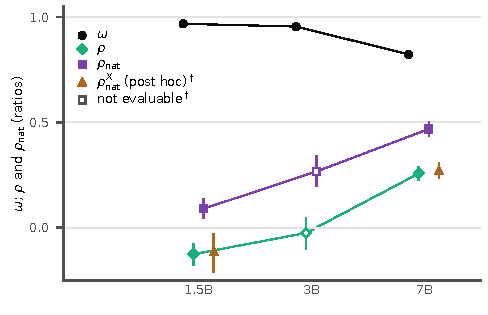
\includegraphics[width=0.5\textwidth]{figures/fig_flag_scale.pdf}
\caption{\textbf{The flag across scale} (Qwen2.5-1.5B, 3B and 7B; 95\,\% story-bootstrap intervals). $\omega$: how far the flag written in a sentence matches the list's; $\rho$ and $\rho_{\mathrm{nat}}$: the injected and the natural sentence-to-list ratio (J-D6, not met: outcome ``Mixed.''); $\rho^X_{\mathrm{nat}}$: the natural ratio on the contrast specific to the absent option (post hoc). Hollow and $\dagger$: not evaluable at 3B, values recomputed.}
\label{fig:flag-scale}
\end{figure}

\paragraph{The flag is written in sentences (J-D6a, replication, held).} At Qwen2.5-1.5B, 3B and 7B the flag written by the reader heads at the sentence's re-mentions matches the list's: $\omega$ = \JdSixaOmegaQwenOnefive{}, \JdSixaOmegaQwenThree{} and \JdSixaOmegaQwenSeven{}, cosine $c_{\mathrm{fl}}$ = \JdSixaKappaQwenOnefive{}, \JdSixaKappaQwenThree{} and \JdSixaKappaQwenSeven{} (\cref{tab:flag}, bottom). The sentence flag injected at the list row moves the answer \JdSixbQwenOnefive{}, \JdSixbQwenThree{} and \JdSixbQwenSeven{} as much as the list flag (reported). The reader heads at 1.5B and 3B were ranked in the final round with the discovery sample's procedure (17 and 29 heads).

\paragraph{Mediation (J-D6, risky, not held; J-D6-ROUTE, risky, not held).} J-D6 predicted that the list flag injected at the sentence's row of the absent option reproduces the natural ratio of the sentence read to the list read, in sign and within $\pm\max(0.1, 0.5\lvert\rho_{\mathrm{nat}}\rvert)$. At 1.5B the signs differ ($\rho$ = \JdSixRhoQwenOnefive{} [\JdSixRhoQwenOnefiveLo{}, \JdSixRhoQwenOnefiveHi{}] against $\rho_{\mathrm{nat}}$ = \JdSixRhoNatQwenOnefive{} [\JdSixRhoNatQwenOnefiveLo{}, \JdSixRhoNatQwenOnefiveHi{}]); at 7B $\rho$ = \JdSixRhoQwenSeven{} against $\rho_{\mathrm{nat}}$ = \JdSixRhoNatQwenSeven{}, a difference of \JdSixDiffQwenSeven{} [\JdSixDiffQwenSevenLo{}, \JdSixDiffQwenSevenHi{}] against a tolerance of $\pm$\JdSixTolQwenSeven{}; 3B is not evaluable (\JdGsixCompQwenThree{} of \JdGsixNQwenThree{} competent cores, against 40). J-D6-ROUTE predicted that at 1.5B the injected flag is read by value under \fmtPost{}; it is read by key ($r^{\mathrm{inj}}(V)$ = \JdSixRouteVQwenOnefive{}, $r^{\mathrm{inj}}(K)$ = \JdSixRouteKQwenOnefive{}, difference \JdSixRouteVmKQwenOnefive{} [\JdSixRouteVmKQwenOnefiveLo{}, \JdSixRouteVmKQwenOnefiveHi{}]). The preregistered decision table gives outcome (\JdSixTable{}), whose text is ``Mixed.'': J-D6 is not met, and $\rho_{\mathrm{nat}}$ is positive in both evaluable models, so the outcome ``not mediated'' does not apply. % verbatim: D6 decision table, entry J part D

\paragraph{A post hoc reading of the natural ratio.} The preregistered $\rho_{\mathrm{nat}}$ divides the natural clamp's effect on X under \fmtPost{} by that under \fmtOpt{}; under \fmtPost{} it includes a gain that every candidate other than B gets when B loses its key match (at 1.5B the clamp to S raises X more than the clamp to X does). On a contrast specific to the absent option (the clamp to X minus the clamp to S, on X), the natural ratio is \JdSixNatXQwenOnefive{} [\JdSixNatXQwenOnefiveLo{}, \JdSixNatXQwenOnefiveHi{}] at 1.5B and \JdSixNatXQwenSeven{} [\JdSixNatXQwenSevenLo{}, \JdSixNatXQwenSevenHi{}] at 7B, and $\rho$ minus it is \JdSixDiffXQwenOnefive{} [\JdSixDiffXQwenOnefiveLo{}, \JdSixDiffXQwenOnefiveHi{}] and \JdSixDiffXQwenSeven{} [\JdSixDiffXQwenSevenLo{}, \JdSixDiffXQwenSevenHi{}]; on the ratio of $\mathrm{ID}_K$, from which the entry's prior was taken, it is \JdSixNatIDKQwenOnefive{} and \JdSixNatIDKQwenSeven{}, and $\rho$ minus it \JdSixDiffIDKQwenOnefive{} [\JdSixDiffIDKQwenOnefiveLo{}, \JdSixDiffIDKQwenOnefiveHi{}] and \JdSixDiffIDKQwenSeven{} [\JdSixDiffIDKQwenSevenLo{}, \JdSixDiffIDKQwenSevenHi{}] (post hoc, recomputed). On these contrasts the injected sentence-row flag reproduces the natural ratio in sign and size, and the decision table would read (b). This reading came after the data and cannot be scored: the verdict stays not met and the outcome (d), and we draw no conclusion about mediation from it in either direction. At 3B, on its 35 competent cores, the line would have failed: $\rho$ = \JdSixRhoQwenThree{} against $\rho_{\mathrm{nat}}$ = \JdSixRhoNatQwenThree{} (post hoc, recomputed). % verbatim: 35 cores, outcome J part D
